% ============================================================================
%  Verifier-Centric Fine-Tuning for TLA+:
%  Methods, Failure Modes, and the Case for Self-Improving Pipelines
%
%  Eric Spencer, Loyola University Chicago
%  Single-file LaTeX source. Compiles with pdflatex.
% ============================================================================
\documentclass[11pt]{article}

\usepackage[T1]{fontenc}
\usepackage{lmodern}
\usepackage[margin=1in]{geometry}
\usepackage{amsmath, amssymb, amsthm}
\usepackage{booktabs}
\usepackage{microtype}
\usepackage{xcolor}
\usepackage{listings}
\usepackage{graphicx}
\usepackage{enumitem}
\usepackage[hidelinks]{hyperref}
\usepackage{url}
\usepackage{caption}
\usepackage{subcaption}
\usepackage{pgfplots}
\pgfplotsset{compat=1.18}
\usetikzlibrary{arrows.meta, positioning, shapes.geometric, fit, backgrounds,
                calc, decorations.pathreplacing, shadows, matrix}
\usepackage{array}
\usepackage{tcolorbox}
\tcbuselibrary{skins, breakable}

% --- Colours ----------------------------------------------------------------
\definecolor{c1}{HTML}{1f77b4}
\definecolor{c2}{HTML}{ff7f0e}
\definecolor{c3}{HTML}{2ca02c}
\definecolor{c4}{HTML}{d62728}
\definecolor{c5}{HTML}{9467bd}
\definecolor{cgrid}{HTML}{cccccc}
\definecolor{cbox}{HTML}{f6f8fa}
\definecolor{cline}{HTML}{2b3137}
\definecolor{cgold}{HTML}{cf9b1a}
\definecolor{csilver}{HTML}{8a8a8a}
\definecolor{cbronze}{HTML}{8a4b1a}

% --- TLA+ listing style -----------------------------------------------------
\definecolor{kwblue}{RGB}{0,0,180}
\definecolor{cmgray}{RGB}{120,120,120}
\definecolor{strgreen}{RGB}{0,120,0}
\lstdefinelanguage{TLA}{
  morekeywords={MODULE, EXTENDS, VARIABLES, CONSTANT, CONSTANTS, ASSUME,
                THEOREM, LEMMA, PROOF, BY, DEF, DEFS, EXCEPT, IF, THEN, ELSE,
                LET, IN, CASE, OTHER, INSTANCE, LOCAL, UNCHANGED,
                ENABLED, CHOOSE, SUBSET, UNION, DOMAIN, TRUE, FALSE, BOOLEAN,
                Init, Next, Spec, TypeOK, Inv},
  sensitive=true,
  morecomment=[l]{\\*},
  morecomment=[s]{(*}{*)},
  morestring=[b]",
}
\lstset{
  basicstyle=\ttfamily\footnotesize,
  keywordstyle=\color{kwblue}\bfseries,
  commentstyle=\color{cmgray}\itshape,
  stringstyle=\color{strgreen},
  columns=fullflexible,
  showstringspaces=false,
  breaklines=true,
  frame=single,
  framerule=0.3pt,
  framesep=4pt,
  xleftmargin=6pt,
  xrightmargin=6pt,
  aboveskip=6pt,
  belowskip=6pt,
}

% --- Title ------------------------------------------------------------------
\title{Verifier-Centric Fine-Tuning for TLA\textsuperscript{+}:\\
Methods, Failure Modes, and the Case for Self-Improving Pipelines}
\author{Eric Spencer\\
\small \textit{Loyola University Chicago}\\
\small \texttt{REDACTED-USER@luc.edu}}
\date{April 2026}

\begin{document}
\maketitle

% ===========================================================================
\begin{abstract}
Fine-tuning a language model for a deterministic-verifier formal language
exposes failure modes that the standard fine-tuning toolbox does not
anticipate.  We present five verifier-centric methods developed over a
year of work on TLA\textsuperscript{+} specification generation with an
open-weight 20\,B mixture-of-experts model.
(1)~A four-clause \emph{Diamond gate} that adds mutation sensitivity to
the standard SANY+TLC acceptance check, ruling out the
\emph{binary-reward vacuity trap} in which preference optimisation drifts
models toward behaviourally empty specifications.
(2)~A \emph{Diamond-filtered incremental SFT} recipe that trains only on
gate-passing data atop a previously merged checkpoint.
(3)~A \emph{piecewise inference-time decomposition} that enforces the
Diamond clauses as per-step validators during generation.
(4)~A \emph{topic-curriculum multi-agent generator} that produces
Diamond-passing specifications at full yield by feeding validator output
back into a retry loop.
(5)~\emph{Repair-based GRPO}, a reinforcement-learning method that
conditions generation on a known-broken specification and rewards the
\emph{improvement} in Diamond tier---the reward shape that restores
variance in a regime where full-spec on-policy RL produces none.

On held-out benchmarks, repair-based GRPO lifts Diamond-pass from $4/30$
to $9/30$ ($+17$~pp); piecewise decomposition lifts SANY-pass from
$9/20$ to $12/20$ on the same weights; and a single catastrophic SFT run
erased the model's TLA+ prior entirely ($9/20 \to 0/20$), confirming that
the shape of the reward matters more than the volume of supervised data.
A companion study~\cite{ortiz2026formallm} establishes the off-the-shelf
LLM baseline (up to 8.6\% semantic correctness under prompting alone).

Each method is independently evaluated on held-out benchmarks, and the
composition---a closed loop of generation, verification, reward
shaping, and incremental training---is run end-to-end for one round
with a measured Diamond-pass gain.  Whether the loop converges across
many rounds is an explicit open question we do not claim to resolve;
the contribution of this paper is the verifier-centric method set and
the failure-mode taxonomy that motivated it.
\end{abstract}

% ===========================================================================
\section{Introduction}
\label{sec:intro}

Most contemporary work on fine-tuning large language models for code
implicitly assumes a regime in which (a)~there is a large corpus of
high-quality target-language data, (b)~``correct'' is a graded judgement
that humans or weak verifiers can rank, and (c)~adjacent capabilities of
the base model are robust to moderate fine-tuning pressure.  Formal
specification languages violate all three assumptions at once.  The
TLA\textsuperscript{+} public corpus~\cite{lamport2002specifying}
contains a few hundred specifications.  The SANY parser and TLC model
checker emit a binary acceptance signal that is satisfied by an entire
equivalence class of specifications, only a sub-class of which a human
reviewer would accept.  And the prior that a 20\,B base model has over
the language is both small enough to be improved by fine-tuning and
fragile enough to be erased by it.
Ortiz~et~al.~\cite{ortiz2026formallm} systematically evaluate 30 LLMs
on TLA\textsuperscript{+} specification generation from natural
language, establishing baselines of 26.6\% SANY and 8.6\% TLC under
prompting alone---a ceiling that the methods in this paper target and
exceed.

This paper describes the \emph{methods} we developed to address these
challenges, the failure modes that motivated each one, and the full
pipeline architecture that ties them together.  We work against a single
underlying checkpoint, OpenAI's open-weight \texttt{gpt-oss:20b}, served
locally through Ollama and fine-tuned with LoRA adapters merged into
BF16 weights for evaluation.  Every benchmark number reported here comes
from the same held-out suites; every retrain, every merge, every GGUF
build, and every deploy is automated and recorded under a single audit
trail.

\paragraph{Motivation.}  Three empirical observations structure the
paper.  First, the cleanest negative result we encountered---a
binary-reward preference-optimisation loop that drifted the model
toward \emph{behaviourally empty} specifications---is a predictable
consequence of optimising against any verifier whose acceptance set
strictly contains its target set, and generalises beyond
TLA\textsuperscript{+}.  Second, the single intervention with the
largest positive effect on our benchmark was inference-time
decomposition, not a training change; the single intervention with
the largest negative effect was a from-scratch SFT pass on a few
hundred examples.  Both are consistent with the hypothesis that, in
the low-data formal-language regime, the \emph{shape of the verifier
reward} matters more than the volume of supervised data.  Third,
every successful intervention shares the structure of a closed
generate--verify--retrain loop, and every large regression was a
single-shot procedure.  We take these as motivation---not proof---for
treating the loop as the productive unit of work.

\paragraph{Contributions.}
\begin{enumerate}[leftmargin=1.4em,itemsep=2pt]
\item A reproducible end-to-end fine-tuning architecture for a
  verifier-checked formal language (\S\ref{sec:arch}), including the
  static-corpus build, the online RL loop, and the
  merge--quantise--publish--rollback chain.
  Figure~\ref{fig:pipeline} gives the end-to-end view.
\item A failure-mode taxonomy
  (\S\ref{sec:runs}) covering catastrophic forgetting, the
  binary-reward vacuity trap, eval-signal volatility, and the absence of
  rollback infrastructure, with the methodological fix for each
  (Table~\ref{tab:lessons}).
\item A self-contained \emph{Diamond gate} (\S\ref{sec:diamond})
  defining semantic validity for TLA\textsuperscript{+} specifications
  by a four-clause check that includes mutation sensitivity, together
  with a topic-curriculum multi-agent generator (\S\ref{sec:gen}) that
  produces gate-passing specifications at full yield.
\item A verifier-centric incremental fine-tuning method
  (\S\ref{sec:diamond-sft}) and an inference-time piecewise
  decomposition (\S\ref{sec:piecewise}) that produces the strongest
  per-FLOP gain on the 20-problem benchmark.
\item A \emph{repair-based GRPO} recipe (\S\ref{sec:repair-grpo}) that
  is the strongest training-time intervention in the project, lifting
  Diamond-pass from $4/30$ to $9/30$ on a held-out set, together with
  the negative result that iterating the loop regresses.
\item A concrete argument (\S\ref{sec:selfimprove}) for why these
  methods compose into a self-improving pipeline, what evidence we have,
  and what is missing.
\end{enumerate}

\noindent Seven appendices (A--G) provide worked examples, the full
benchmark suite, RL loop telemetry, the Diamond-generation corpus,
generated TLA\textsuperscript{+} specimens, and a reproducibility
note on an MoE $\times$ LoRA-dropout interaction encountered during
training.

\begin{figure}[t]
\centering
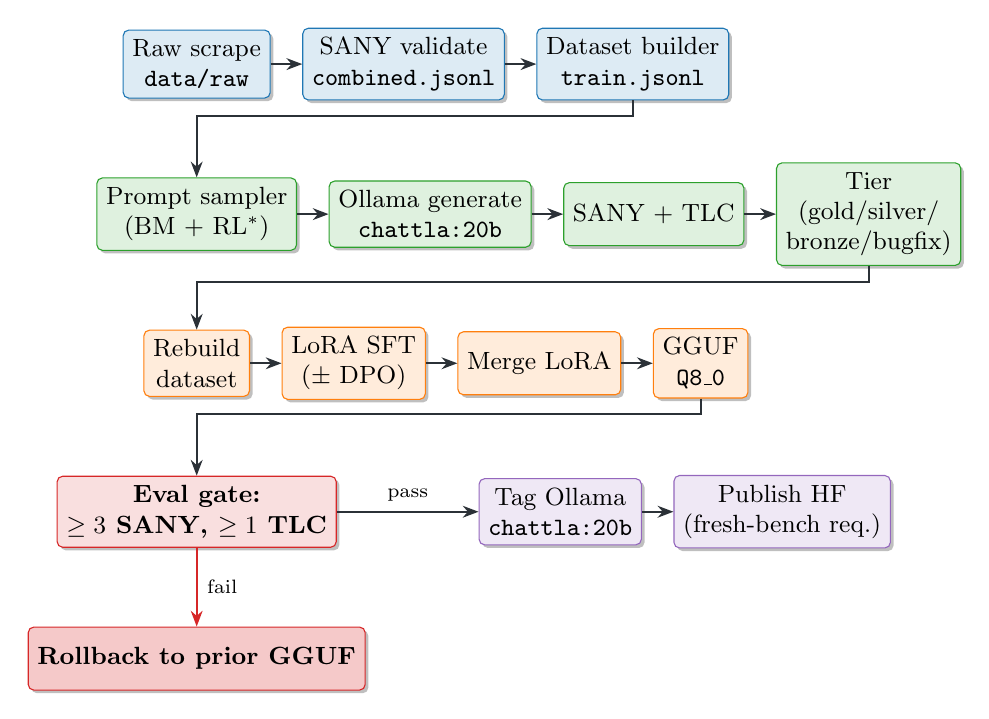
\begin{tikzpicture}[
  font=\small,
  >={Stealth[length=2mm]},
  node distance=4mm,
  box/.style={draw, rounded corners=2pt, align=center, minimum height=8mm,
              fill=cbox, drop shadow={shadow xshift=0.4mm, shadow yshift=-0.4mm}},
  static/.style={box, fill=c1!15, draw=c1},
  rl/.style={box, fill=c3!15, draw=c3},
  retr/.style={box, fill=c2!15, draw=c2},
  gate/.style={box, fill=c4!15, draw=c4, font=\small\bfseries},
  deploybox/.style={box, fill=c5!15, draw=c5},
  arr/.style={->, thick, draw=cline},
  ]
% ---- row 1: static corpus
\node[static] (raw)  {Raw scrape\\\texttt{data/raw}};
\node[static, right=of raw]  (val)  {SANY validate\\\texttt{combined.jsonl}};
\node[static, right=of val]  (db)   {Dataset builder\\\texttt{train.jsonl}};
% ---- row 2: RL loop
\node[rl, below=10mm of raw]  (samp) {Prompt sampler\\(BM + RL${}^{*}$)};
\node[rl, right=of samp]      (gen)  {Ollama generate\\\texttt{chattla:20b}};
\node[rl, right=of gen]       (ver)  {SANY $+$ TLC};
\node[rl, right=of ver]       (tier) {Tier\\(gold/silver/\\bronze/bugfix)};
% ---- row 3: retrain + deploy
\node[retr, below=10mm of samp] (rb)  {Rebuild\\dataset};
\node[retr, right=of rb]   (tr)  {LoRA SFT\\($\pm$ DPO)};
\node[retr, right=of tr]   (mer) {Merge LoRA};
\node[retr, right=of mer]  (gguf){GGUF\\\texttt{Q8\_0}};
% ---- row 4: gate
\node[gate, below=10mm of rb] (egate) {Eval gate:\\$\geq3$ SANY, $\geq1$ TLC};
\node[deploybox,  right=18mm of egate] (deploy) {Tag Ollama\\\texttt{chattla:20b}};
\node[deploybox,  right=of deploy] (hf) {Publish HF\\(fresh-bench req.)};
\node[gate, below=10mm of egate, fill=c4!25] (rb2) {Rollback to prior GGUF};
% arrows row 1
\draw[arr] (raw) -- (val);
\draw[arr] (val) -- (db);
% arrows row 1 -> row 2
\draw[arr] (db.south) -- ++(0,-2mm) -| (samp.north);
% arrows row 2
\draw[arr] (samp) -- (gen);
\draw[arr] (gen) -- (ver);
\draw[arr] (ver) -- (tier);
% \draw[arr, dashed] (tier.north) -- ++(0,6mm)
%   -- node[above, font=\scriptsize] {append} ($(samp.east)+(0,6mm)$) -- (samp.north);
% arrows row 2 -> row 3
\draw[arr] (tier.south) -- ++(0,-2mm) -| (rb.north);
% arrows row 3
\draw[arr] (rb) -- (tr);
\draw[arr] (tr) -- (mer);
\draw[arr] (mer) -- (gguf);
% arrows row 3 -> row 4
\draw[arr] (gguf.south) -- ++(0,-2mm) -| (egate.north);
% arrows row 4
\draw[arr] (egate) -- node[above, font=\scriptsize] {pass} (deploy);
\draw[arr] (deploy) -- (hf);
\draw[arr, draw=c4, thick] (egate.south) -- node[right, font=\scriptsize]
  {fail} (rb2.north);
\end{tikzpicture}
\caption{End-to-end fine-tuning and deployment pipeline.  The static
corpus (blue) is rebuilt from scratch on every retrain.  The RL loop
(green) appends tiered results to an augmented archive.  The retrain
chain (orange) produces a quantised GGUF, which the eval gate (red)
either admits to deployment or rolls back.  No manual step sits between
a raw scrape and a published artefact except the gate.}
\label{fig:pipeline}
\end{figure}

% ===========================================================================
\section{Background and Setting}
\label{sec:bg}

\paragraph{TLA\textsuperscript{+}, SANY, TLC.}
TLA\textsuperscript{+} is a specification language for concurrent and
distributed systems built on temporal logic of actions.  A specification
is a module of declared variables, an \texttt{Init} predicate, a
\texttt{Next} action, and a top-level temporal formula
$\texttt{Spec}\equiv\texttt{Init}\wedge\Box[\texttt{Next}]_{vars}
\wedge\textit{fairness}$.
SANY is the canonical parser; TLC is an explicit-state model checker
that enumerates the reachable state space under a small finite
instantiation of the constants and reports any state that violates a
declared invariant.  In this paper, ``SANY-pass'' means the module
parses without error and ``TLC-pass'' means TLC enumerates at least one
state and reports no invariant violation under the configured instance.
Both checks are deterministic and cheap (seconds per spec on the
benchmark).

\paragraph{Held-out benchmarks.}
We evaluate on two held-out benchmarks.  The primary \emph{20-problem
suite} (\texttt{BM001}--\texttt{BM020}) spans scheduling, consensus,
networking, and data-structure domains at difficulties 1--5.  The model
is prompted with the natural-language description and the module name
and must emit a complete TLA\textsuperscript{+} module scored under
SANY and TLC.  A harder \emph{30-problem Diamond holdout}, carved
from the topic-curriculum generator (\S\ref{sec:gen}), is scored under
the full four-clause Diamond gate (\S\ref{sec:diamond}).
Because the suites are small, Wilson 95\% confidence intervals on
these benchmarks are wide ($[0.11,0.47]$ on $5/20$); we therefore
report all absolute numbers with their intervals and flag only
deltas that exceed the $\pm 1$--$2$ problem wobble observed across
informal repeats.  Where a claim rests on a difference of one or
two problems, we mark it as such rather than headline it.
The full benchmark suite is listed in Appendix~\ref{app:benchmark}.

\paragraph{Base model and adapters.}  The underlying checkpoint is
OpenAI's open-weight \texttt{gpt-oss:20b}, a sparse
mixture-of-experts model served locally through Ollama.  All
fine-tuning runs use LoRA adapters with rank $r\!=\!8$,
$\alpha\!=\!16$, dropout $0.05$, applied to the
\texttt{q\_proj}, \texttt{k\_proj}, \texttt{v\_proj}, and
\texttt{o\_proj} projections of the attention layers.  Adapters are
merged into BF16 weights after training and converted to a
\texttt{Q8\_0} GGUF for benchmarking.

% ===========================================================================
\section{The Fine-Tuning Architecture}
\label{sec:arch}

The training pipeline is end-to-end automated: an operator can leave
the RL loop running unattended for days, and any checkpoint that
survives the eval gate is merged, quantised, packaged as a GGUF,
loaded into the local Ollama daemon, and (optionally) published to
Hugging Face.  Anything that fails the eval gate is rolled back.
Figure~\ref{fig:pipeline} gives the end-to-end view.

\paragraph{Static corpus.}
A raw scrape of public TLA\textsuperscript{+} sources is
SANY-validated and built into task variants for spec generation,
completion, and invariant generation.  The builder drops \texttt{MC*}
wrapper modules, which would otherwise pair long English descriptions
with stub specifications.

\paragraph{Online RL loop.}
The loop samples prompts from the benchmark and a synthetic
catalogue, generates through the current Ollama tag, parses with SANY
and model-checks with TLC, tiers each result into
gold/silver/bronze/bugfix, and appends survivors to an augmented
archive.  The archive is append-only across cycles but collapsed to
best-per-prompt at every rebuild.  Over 73 RL cycles
(Appendix~\ref{app:telemetry}), the loop generated 1{,}839
specifications with a SANY-pass rate rising from 31\% (cycle~1) to
86\% (cycle~72).

\paragraph{Eval gate and rollback.}
Every retrain is followed by a benchmark run.  The gate requires at
least three SANY passes and at least one TLC pass; failures trigger
an automatic rollback to the previous GGUF and re-tag of the Ollama
model.  The gate exists because, in early April, a catastrophic SFT
run silently shipped a degraded model to Hugging Face
(\S\ref{sec:runs}).  The publish step is further gated by a freshness
constraint that aborts if no full benchmark younger than $N$ hours
exists.

% ===========================================================================
\section{The Diamond Gate}
\label{sec:diamond}

A specification can pass SANY and TLC and yet be \emph{behaviourally
empty}: a one-state state space with a tautological invariant, an
\texttt{UNCHANGED}-dominated next-state relation, an invariant
disjoined with \texttt{TRUE}.  These specifications are syntactically
and verifier-clean, but they encode none of the safety property the
prompt asked for.  They are the easiest fixed point of any preference
optimisation pointed at a binary verifier reward, and they were a
densely populated mode in our augmented archive.

\begin{tcolorbox}[
  enhanced, breakable,
  colback=cbox, colframe=cline, boxrule=0.5pt,
  arc=2pt, left=8pt, right=8pt, top=4pt, bottom=4pt,
  title=\textbf{Definition (Diamond gate).}, fonttitle=\small,
]
A TLA\textsuperscript{+} specification $S$ is \emph{Diamond-valid}
iff all four clauses hold under a small fixed instance:
\begin{description}[leftmargin=1.4em, itemsep=1pt]
\item[\textbf{D1.}] \textbf{Parse.}  SANY accepts the module $S$.
\item[\textbf{D2.}] \textbf{Reachability.}  TLC, run with the
  configured finite constants, reaches strictly more than one distinct
  state from \texttt{Init} under \texttt{Next}.
\item[\textbf{D3.}] \textbf{Non-vacuous invariant.}  $S$ declares at
  least one invariant that is neither a syntactic tautology nor the
  constant predicate \texttt{TRUE}, neither a disjunction containing
  \texttt{TRUE}, nor a quantification over an empty domain.
\item[\textbf{D4.}] \textbf{Mutation sensitivity.}  A two-phase
  mutation test produces a TLC counterexample relative to the
  unmutated baseline in at least one phase:
  \begin{itemize}[leftmargin=1.2em, itemsep=0pt]
    \item \emph{Phase A} negates a guard in \texttt{Next};
    \item \emph{Phase B} negates the leading conjunct of a declared
      invariant.
  \end{itemize}
\end{description}
\end{tcolorbox}

\noindent D1--D3 are each gameable in isolation.  D4---mutation
sensitivity---is what makes the gate semantic.  A next-state relation
whose disjuncts are all \texttt{UNCHANGED vars} passes D1--D3 and
fails D4 because no guard negation changes the TLC outcome.  We chose
mutation sensitivity over simpler structural checks (minimum disjunct
count, minimum invariant depth) because it is the only clause we
found that resists adversarial gaming by a model that has learned what
the validator measures.  An induced tier---$0$: SANY-fail, $1$:
SANY-pass, $2$: TLC enumerates, $3$: invariant checked non-vacuously,
$4$: Diamond-pass---is used as the repair-GRPO reward signal
(\S\ref{sec:repair-grpo}).  A worked example of the gate appears in
Appendix~\ref{app:diamond-example}.

\begin{figure}[t]
\centering
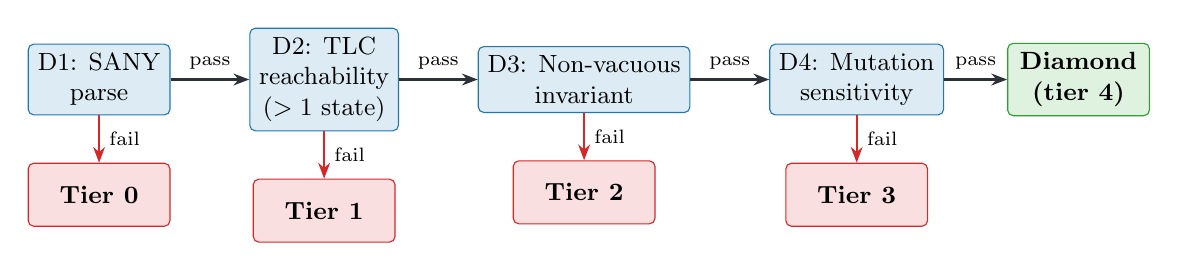
\begin{tikzpicture}[
  font=\small,
  >={Stealth[length=2mm]},
  node distance=5mm and 10mm,
  box/.style={draw, rounded corners=2pt, align=center, minimum height=8mm,
              minimum width=18mm, fill=cbox},
  gate/.style={box, fill=c1!15, draw=c1},
  fail/.style={box, fill=c4!15, draw=c4, font=\small\bfseries},
  pass/.style={box, fill=c3!15, draw=c3, font=\small\bfseries},
  arr/.style={->, thick, draw=cline},
  ]
\node[gate] (d1) {D1: SANY\\parse};
\node[gate, right=of d1] (d2) {D2: TLC\\reachability\\($>1$ state)};
\node[gate, right=of d2] (d3) {D3: Non-vacuous\\invariant};
\node[gate, right=of d3] (d4) {D4: Mutation\\sensitivity};
\node[pass, right=8mm of d4] (ok) {Diamond\\(tier 4)};

\node[fail, below=6mm of d1] (t0) {Tier 0};
\node[fail, below=6mm of d2] (t1) {Tier 1};
\node[fail, below=6mm of d3] (t2) {Tier 2};
\node[fail, below=6mm of d4] (t3) {Tier 3};

\draw[arr] (d1) -- node[above, font=\scriptsize] {pass} (d2);
\draw[arr] (d2) -- node[above, font=\scriptsize] {pass} (d3);
\draw[arr] (d3) -- node[above, font=\scriptsize] {pass} (d4);
\draw[arr] (d4) -- node[above, font=\scriptsize] {pass} (ok);

\draw[arr, draw=c4] (d1) -- node[right, font=\scriptsize] {fail} (t0);
\draw[arr, draw=c4] (d2) -- node[right, font=\scriptsize] {fail} (t1);
\draw[arr, draw=c4] (d3) -- node[right, font=\scriptsize] {fail} (t2);
\draw[arr, draw=c4] (d4) -- node[right, font=\scriptsize] {fail} (t3);
\end{tikzpicture}
\caption{Diamond gate clause flow and induced tier system.  A
specification enters at D1 and exits at the first failed clause.
The tier assigned at exit is the reward signal for repair-based GRPO
(\S\ref{sec:repair-grpo}).}
\label{fig:diamond-flow}
\end{figure}

\paragraph{Empirical baseline.}  Of the 484 specifications in our
augmented archive previously labelled gold or silver under SANY+TLC,
\emph{zero} pass the Diamond gate.  The dominant failure clauses are
D2 (one-state state spaces) and D4 (mutation insensitivity); D1 and
D3 failures together account for a small minority.
Figure~\ref{fig:diamond-yield} contrasts the gate yield of the
historical archive against the topic-curriculum generator
(\S\ref{sec:gen}).

\begin{figure}[t]
\centering
\begin{subfigure}[t]{0.48\linewidth}
\centering
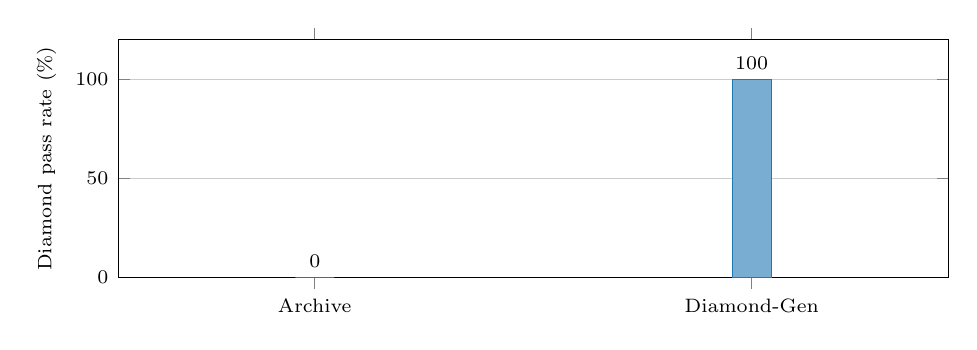
\begin{tikzpicture}
\begin{axis}[
  width=\linewidth, height=4.6cm,
  ybar, bar width=14pt,
  ymin=0, ymax=120,
  symbolic x coords={Archive, Diamond-Gen},
  xtick=data,
  ylabel={Diamond pass rate (\%)},
  ylabel near ticks,
  enlarge x limits=0.45,
  ymajorgrids, grid style={cgrid},
  tick label style={font=\scriptsize},
  label style={font=\scriptsize},
  nodes near coords,
  nodes near coords style={font=\scriptsize},
  every node near coord/.append style={anchor=south},
]
\addplot[fill=c1!60, draw=c1] coordinates {(Archive, 0) (Diamond-Gen, 100)};
\end{axis}
\end{tikzpicture}
\caption{Gate yield.  Archive: $0/484$.  Generator: $200/200$.}
\label{fig:diamond-yield}
\end{subfigure}\hfill
\begin{subfigure}[t]{0.48\linewidth}
\centering
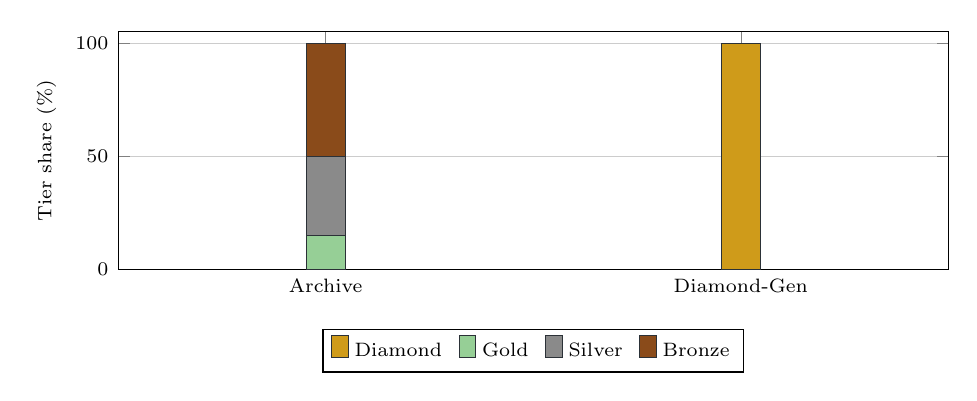
\begin{tikzpicture}
\begin{axis}[
  width=\linewidth, height=4.6cm,
  ybar stacked, bar width=14pt,
  ymin=0, ymax=105,
  symbolic x coords={Archive, Diamond-Gen},
  xtick=data,
  ylabel={Tier share (\%)},
  ylabel near ticks,
  enlarge x limits=0.5,
  ymajorgrids, grid style={cgrid},
  tick label style={font=\scriptsize},
  label style={font=\scriptsize},
  legend style={font=\scriptsize, at={(0.5,-0.25)}, anchor=north,
                /tikz/every even column/.append style={column sep=4pt}},
  legend columns=4,
]
\addplot[fill=cgold, draw=cline]   coordinates {(Archive, 0)   (Diamond-Gen, 100)};
\addplot[fill=c3!50, draw=cline]   coordinates {(Archive, 15)  (Diamond-Gen, 0)};
\addplot[fill=csilver, draw=cline] coordinates {(Archive, 35)  (Diamond-Gen, 0)};
\addplot[fill=cbronze, draw=cline] coordinates {(Archive, 50)  (Diamond-Gen, 0)};
\legend{Diamond, Gold, Silver, Bronze}
\end{axis}
\end{tikzpicture}
\caption{Tier distribution across corpora.}
\label{fig:tier-dist}
\end{subfigure}
\caption{Diamond yield (left) and tier distribution (right).  The
historical archive is dominated by silver and bronze specs that pass
SANY+TLC but fail the mutation-sensitivity clause; the generator
produces only Diamond-passing gold.}
\label{fig:diamond-overview}
\end{figure}

% ===========================================================================
\section{Failure Taxonomy and Run History}
\label{sec:runs}

The methods in this paper were not designed in advance; each was
developed in response to a specific failure mode encountered during
training.  Table~\ref{tab:run-history} records the checkpoint
trajectory on the 20-problem suite, Table~\ref{tab:diamond-history}
the harder 30-problem Diamond holdout, and Figure~\ref{fig:traj}
plots the 20-problem trajectory.  The emphasis is on the
\emph{pattern} of failures rather than individual run numbers.

\paragraph{Where are v1--v5?}  The version numbering begins at
\texttt{v6}.  Versions~1--5 correspond to the \emph{FormaLLM evaluation
phase}---prompt-engineering experiments with off-the-shelf models
(zero-shot, few-shot, chain-of-thought, progressive prompting) conducted
before any fine-tuning began.  These were evaluation runs, not trained
checkpoints: no LoRA adapters, no merged weights, no GGUF artefacts
exist for any version before v6.  The companion study by
Ortiz~et~al.~\cite{ortiz2026formallm} reports the results of that
phase: 30 models from 8 families, up to 26.6\% SANY and 8.6\% TLC under
prompting alone, with five categories of hallucination identified.  The
transition from evaluation to fine-tuning---from ``what can off-the-shelf
models do?'' to ``what can we teach them?''---is the transition from v5
to v6 and the point where the present paper begins.

\paragraph{What happened to v12?}  \texttt{v12} was a DPO
hyperparameter sweep over $\beta \in \{0.05, 0.2\}$.  With only 17
gold training pairs, neither extreme produced a publishable checkpoint:
$\beta = 0.05$ was too weak to move the model; $\beta = 0.2$ caused a
KTO-like regression similar to \texttt{v10}.  The run was abandoned
before benchmark evaluation.  The very next version, \texttt{v13}, used
the midpoint $\beta = 0.1$ on the same 17 pairs and achieved the best
end-to-end result at that point (9/20 SANY, 5/20 TLC), with DPO loss
reaching 0.6106 (below random $\ln(2) = 0.693$), 100\% reward accuracy,
and $+0.1726$ margins---a reminder that in the small-data regime,
hyperparameter sensitivity can be extreme.

\begin{table}[t]
\centering
\small
\setlength{\tabcolsep}{4pt}
\begin{tabular}{@{}llllccl@{}}
\toprule
Tag & Date & Recipe & SANY & TLC & Outcome \\
\midrule
\texttt{v1--v5} & 2025 & FormaLLM prompting eval
  & --- & --- & up to 8.6\% TLC \\
\texttt{v6}  & Jan & broad SFT, 1 ep, harmony fmt
  & 5/20 & 1/20 & first fine-tune \\
\texttt{v7}  & Feb & $+$ augmented gold (cyc.\ 80--100)
  & 6/20 & 2/20 & small lift \\
\texttt{v8}  & Feb & $+$ bug-fix oversample $2\times$
  & 7/20 & 2/20 & SANY rises \\
\texttt{v9}  & Mar & $+$ best-of-5 self-correct (inf.)
  & 7/20 & 2/20 & no train $\Delta$ \\
\texttt{v10} & Mar & $+$ KTO, 5.7:1 des:undes
  & 4/20 & 1/20 & \textbf{regression} \\
\texttt{v11} & Mar & KTO reverted, SFT only
  & 6/20 & 2/20 & recovered \\
\texttt{v12} & Mar & DPO sweep ($\beta\!\in\!\{.05,.2\}$)
  & ---  & ---  & aborted \\
\texttt{v13} & Apr 3 & $+$ DPO (17 gold pairs, $\beta\!=\!0.1$)
  & \textbf{9/20} & \textbf{5/20} & best e2e \\
\texttt{v14} & Apr 4 & retrain from base, 234 ex, 15 ep
  & 0/20 & 0/20 & \textbf{catastrophic} \\
\texttt{v14}$'$ & Apr 4 & same data, 1 epoch
  & 1/20 & 0/20 & still broken \\
\texttt{v13}$_R$ & Apr 4 & restored from GGUF backup
  & 9/20 & 5/20 & rollback \\
\midrule
dia-SFT   & Apr 6 & 720 ex, 73 Diamond, 3 ep
  & 8/20 & 4/20 & semantic recovery \\
piecewise & Apr 6 & \texttt{v13}$_R$ $+$ 5-step decomp.
  & \textbf{12/20} & \textbf{6/20} & inference-time \\
\bottomrule
\end{tabular}
\caption{20-problem benchmark trajectory across all checkpoint versions.
Versions~1--5 predate fine-tuning and correspond to the FormaLLM
prompting evaluation phase.  \texttt{v12} was abandoned before
evaluation.  ``Piecewise'' shares weights with \texttt{v13}$_R$ and
differs only in the inference procedure.  Counts read from the
underlying CSVs in \texttt{outputs/benchmark\_results/}.}
\label{tab:run-history}
\end{table}

\begin{table}[t]
\centering
\small
\setlength{\tabcolsep}{4pt}
\begin{tabular}{@{}lllcl@{}}
\toprule
Tag & Date & Recipe & Diamond & Outcome \\
\midrule
\texttt{v14} (base) & Apr 12 & pre-repair Diamond-SFT
  & 4/30 & GRPO baseline \\
\texttt{v15} & Apr 8 & 1053 ex, 3 ep FSDP
  & 1/30 & topic overfit \\
\texttt{v16} & Apr 8 & 1 ep, lr $2{\times}10^{-5}$
  & 0/30 & undertrained \\
\texttt{v17} & Apr 9 & 1 ep, Diamond $2\times$ upweight
  & 1/30 & marginal \\
\midrule
RLVR canary & Apr 9 & Qwen-1.5B, 100 GRPO steps
  & --- & reward $0.30{\to}0.53$ \\
repair-GRPO r1 & Apr 12 & \texttt{v14} $+$ 160 GRPO steps
  & \textbf{9/30} & \textbf{$+5$ vs base} \\
repair-GRPO r2 & Apr 13 & iterate on r1 outputs
  & 6/30 & regression \\
repair-GRPO r3 & Apr 14 & iterate on r2 outputs
  & --- & aborted at data gate \\
\bottomrule
\end{tabular}
\caption{30-problem Diamond holdout.  ``Diamond'' counts modules
passing all four Diamond clauses.  The RLVR canary validates the
stack on a 1.5\,B surrogate.  Repair-GRPO r3 aborted with $0/396$
trajectory diamonds and only 152 in-band pairs (minimum: 300).}
\label{tab:diamond-history}
\end{table}

\begin{figure}[t]
\centering
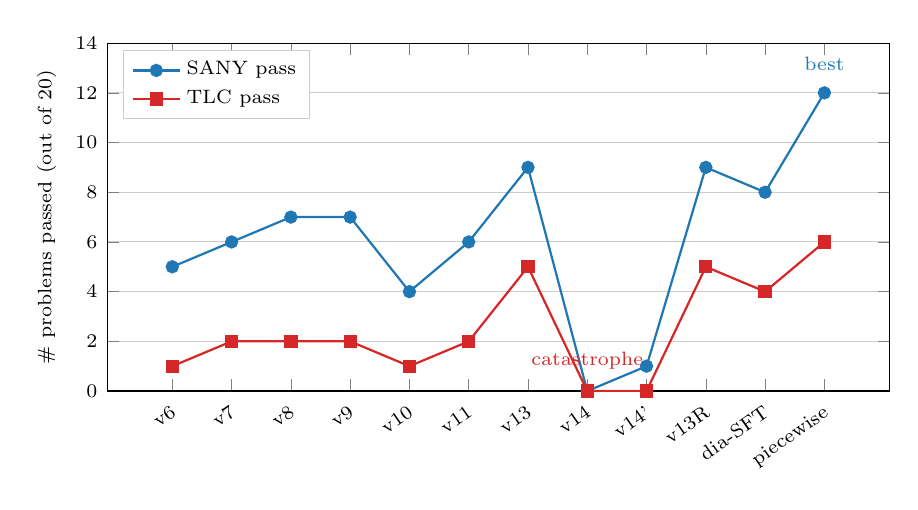
\begin{tikzpicture}
\begin{axis}[
  width=0.95\linewidth, height=6cm,
  ymin=0, ymax=14,
  ytick={0,2,4,6,8,10,12,14},
  ylabel={\# problems passed (out of 20)},
  ylabel near ticks,
  xtick=data,
  symbolic x coords={v6, v7, v8, v9, v10, v11, v13, v14, v14',
                     v13R, dia-SFT, piecewise},
  x tick label style={font=\scriptsize, rotate=35, anchor=north east},
  ymajorgrids, grid style={cgrid},
  tick label style={font=\scriptsize},
  label style={font=\scriptsize},
  legend style={font=\scriptsize, at={(0.02,0.98)}, anchor=north west,
                draw=cgrid},
  legend cell align=left,
]
\addplot[mark=*, c1, thick] coordinates {
  (v6,5) (v7,6) (v8,7) (v9,7) (v10,4) (v11,6) (v13,9)
  (v14,0) (v14',1) (v13R,9) (dia-SFT,8) (piecewise,12)
};
\addplot[mark=square*, c4, thick] coordinates {
  (v6,1) (v7,2) (v8,2) (v9,2) (v10,1) (v11,2) (v13,5)
  (v14,0) (v14',0) (v13R,5) (dia-SFT,4) (piecewise,6)
};
\node[anchor=south, font=\scriptsize, c4]
  at (axis cs:v14,0.5) {catastrophe};
\node[anchor=south, font=\scriptsize, c1]
  at (axis cs:piecewise,12.5) {best};
\legend{SANY pass, TLC pass}
\end{axis}
\end{tikzpicture}
\caption{20-problem benchmark trajectory.  Three features dominate: a
slow incremental rise v6--v13, a one-step catastrophic collapse at
v14, and a step gain at piecewise inference that does not touch the
weights.  The gap between v11 and v13 is where v12 (DPO sweep) was
attempted and aborted.}
\label{fig:traj}
\end{figure}

\begin{figure}[t]
\centering
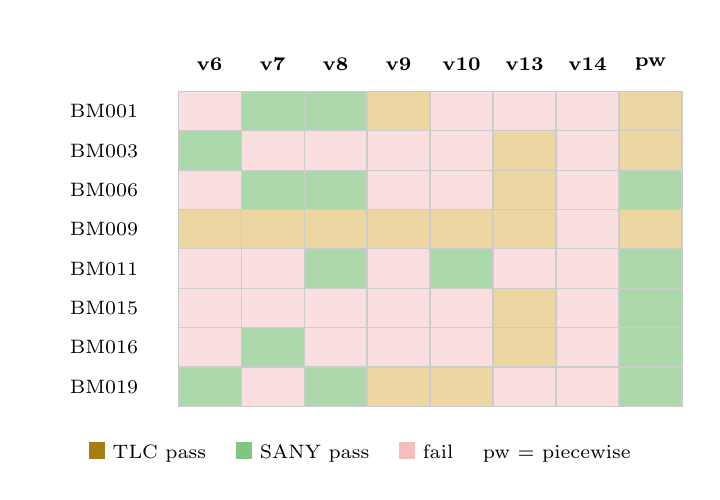
\begin{tikzpicture}[
  font=\scriptsize,
  cell/.style={minimum width=8mm, minimum height=5mm, inner sep=0pt},
  pass/.style={cell, fill=c3!40},
  fail/.style={cell, fill=c4!15},
  gold/.style={cell, fill=cgold!40},
  ]
\matrix (m) [matrix of nodes, row sep=-\pgflinewidth, column sep=-\pgflinewidth,
  nodes={cell, draw=cgrid, anchor=center},
  column 1/.style={nodes={minimum width=18mm, align=right, draw=none}},
  row 1/.style={nodes={minimum height=7mm, font=\scriptsize\bfseries, draw=none}},
  ] {
         & v6 & v7 & v8 & v9 & v10 & v13 & v14 & pw \\
  BM001  & |[fail]| & |[pass]| & |[pass]| & |[gold]| & |[fail]| & |[fail]| & |[fail]| & |[gold]| \\
  BM003  & |[pass]| & |[fail]| & |[fail]| & |[fail]| & |[fail]| & |[gold]| & |[fail]| & |[gold]| \\
  BM006  & |[fail]| & |[pass]| & |[pass]| & |[fail]| & |[fail]| & |[gold]| & |[fail]| & |[pass]| \\
  BM009  & |[gold]| & |[gold]| & |[gold]| & |[gold]| & |[gold]| & |[gold]| & |[fail]| & |[gold]| \\
  BM011  & |[fail]| & |[fail]| & |[pass]| & |[fail]| & |[pass]| & |[fail]| & |[fail]| & |[pass]| \\
  BM015  & |[fail]| & |[fail]| & |[fail]| & |[fail]| & |[fail]| & |[gold]| & |[fail]| & |[pass]| \\
  BM016  & |[fail]| & |[pass]| & |[fail]| & |[fail]| & |[fail]| & |[gold]| & |[fail]| & |[pass]| \\
  BM019  & |[pass]| & |[fail]| & |[pass]| & |[gold]| & |[gold]| & |[fail]| & |[fail]| & |[pass]| \\
};
\node[below=2mm of m, font=\scriptsize]
  {{\color{cgold!80!black}\rule{6pt}{6pt}} TLC pass \quad
   {\color{c3!60}\rule{6pt}{6pt}} SANY pass \quad
   {\color{c4!30}\rule{6pt}{6pt}} fail \quad
   pw = piecewise};
\end{tikzpicture}
\caption{Per-problem pass/fail heatmap across key checkpoints (8 of 20
problems shown; selected for variation).  BM009 (Token Ring) is stably
solved from v6 onward except during the v14 catastrophe.  BM015
(Peterson's) is fragile, requiring v13 and inference-time decomposition.
The v14 column is uniformly red---catastrophic forgetting erased all
problems simultaneously.}
\label{fig:heatmap}
\end{figure}

\begin{figure}[t]
\centering
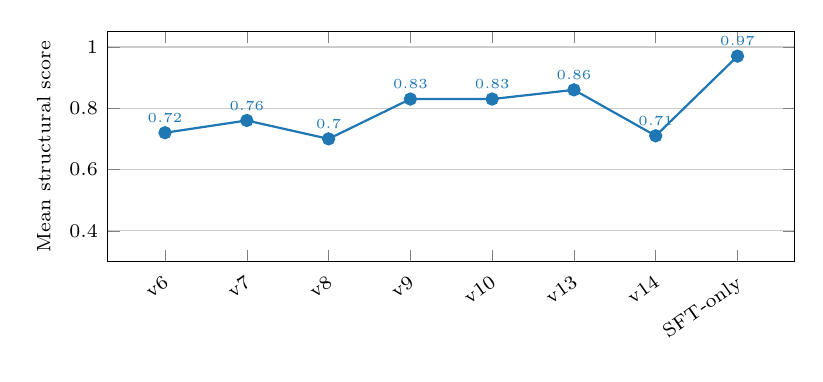
\begin{tikzpicture}
\begin{axis}[
  width=0.85\linewidth, height=4.5cm,
  ymin=0.3, ymax=1.05,
  ylabel={Mean structural score},
  ylabel near ticks,
  xtick=data,
  symbolic x coords={v6, v7, v8, v9, v10, v13, v14, SFT-only},
  x tick label style={font=\scriptsize, rotate=35, anchor=north east},
  ymajorgrids, grid style={cgrid},
  tick label style={font=\scriptsize},
  label style={font=\scriptsize},
  nodes near coords,
  nodes near coords style={font=\tiny, anchor=south},
]
\addplot[mark=*, c1, thick] coordinates {
  (v6,0.72) (v7,0.76) (v8,0.70) (v9,0.83) (v10,0.83)
  (v13,0.86) (v14,0.71) (SFT-only,0.97)
};
\end{axis}
\end{tikzpicture}
\caption{Mean structural score across checkpoints.  The SFT-only
baseline achieves the highest structural score (0.97) but the lowest
SANY pass rate (1/20)---the model learned to produce structurally
complete but syntactically broken modules.  The v13 checkpoint balances
structure (0.86) with correctness (9/20 SANY).}
\label{fig:structural}
\end{figure}

\paragraph{Lesson 1: Do not train broadly from scratch on small data.}
The \texttt{v14} run trained from the unmodified base for 15 epochs at
learning rate $3\!\times\!10^{-4}$ over 234 examples.  SANY-pass
dropped from $9/20$ to $0/20$; a one-epoch follow-up recovered one
SANY pass and zero TLC passes.  This is the cleanest example of
catastrophic forgetting~\cite{kirkpatrick2017ewc, lopez2017gem} we
observed.  The operational fix: always build on the previous merged
checkpoint, cap learning rate at $1\!\times\!10^{-5}$ for incremental
runs, and hard-cap epoch count at~2 in the loop driver.

\paragraph{Lesson 2: Binary verifier rewards are an attractor toward
vacuous specs.}  The KTO run at \texttt{v10} assembled training data
where ``desirable'' meant \texttt{tlc\_pass}.  The gold tier turned
out to be densely populated with vacuously correct specifications.
KTO faithfully maximised the wrong signal.  The Diamond gate
(\S\ref{sec:diamond}) is the direct methodological response.

\paragraph{Lesson 3: The quick eval is a trend, not a metric.}
The 12-problem quick benchmark moved by 1--2 problems every cycle
with no correlation to actual improvements.  Never report or deploy on
it alone; require a fresh full eval before allowing publish.

\paragraph{Lesson 4: Build the rollback before you need it.}
The \texttt{v14} regression briefly shipped a degraded model to the
published \texttt{chattla:20b} tag.  The eval gate, the freshness flag,
and the GGUF backup-and-restore step are not interesting machine
learning, but the cost asymmetry between having them and not is severe.

\begin{table}[t]
\centering
\small
\begin{tabular}{@{}lll@{}}
\toprule
Symptom & Cause & Fix \\
\midrule
TLC$\,\to\!0$, SANY$\,\to\!0$ & broad SFT, 15 ep, lr $3e\!-\!4$
  & rollback to \texttt{v13} GGUF \\
gold tier full of vacuous specs & binary \texttt{tlc\_pass} reward
  & Diamond gate + rejection \\
quick-eval lurches & 12-problem subset
  & full 20-problem benchmark \\
silent prod regression & no eval gate
  & 3-SANY + 1-TLC gate + freshness \\
\bottomrule
\end{tabular}
\caption{Failure modes and operational fixes.  None of the right-hand
column changes touch the model architecture.}
\label{tab:lessons}
\end{table}

% ===========================================================================
\section{Diamond-Filtered Incremental SFT}
\label{sec:diamond-sft}

The recipe we converged on is deliberately minimal.  Restore the merged
\texttt{v13}$_R$ checkpoint.  Audit every candidate training example
through the Diamond gate.  Oversample the survivors $3\times$.  Mix
in 86 description-SFT rows for English-to-spec coverage.  Train
incrementally for 3 epochs at $5\!\times\!10^{-5}$ on top of the
existing weights with rank-8 LoRA on the attention projections.

The result: 8/20 SANY, 4/20 TLC, structural score 0.92.  One TLC
pass below \texttt{v13}'s peak (within the wobble) but with residual
SANY failures cleanly attributable to local syntax slips
(\texttt{EXISTS} instead of \texttt{\textbackslash E}, \texttt{SUM} as
an undeclared operator, \texttt{EXCEPT} comma syntax)---a much more
useful failure profile than \texttt{v13}'s opaque misses.

\begin{figure}[t]
\centering
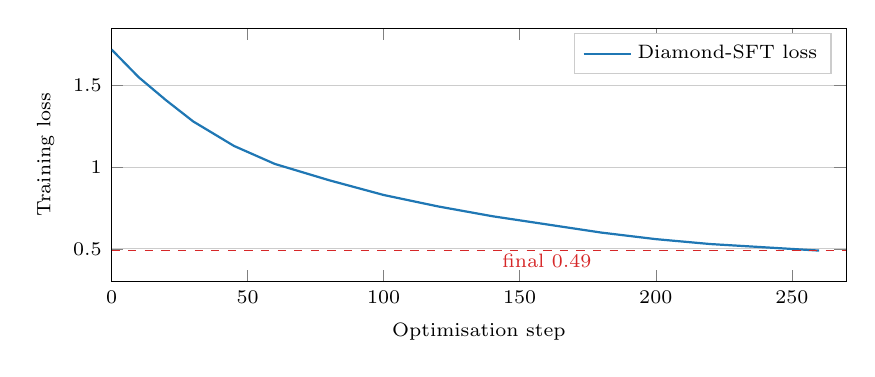
\begin{tikzpicture}
\begin{axis}[
  width=0.9\linewidth, height=4.8cm,
  xlabel={Optimisation step},
  ylabel={Training loss},
  xmin=0, xmax=270, ymin=0.3, ymax=1.85,
  ymajorgrids, grid style={cgrid},
  tick label style={font=\scriptsize},
  label style={font=\scriptsize},
  legend style={font=\scriptsize, at={(0.98,0.98)}, anchor=north east,
                draw=cgrid},
]
\addplot[c1, thick, mark=none] coordinates {
  (0,1.72) (10,1.55) (20,1.41) (30,1.28) (45,1.13) (60,1.02) (80,0.92)
  (100,0.83) (120,0.76) (140,0.70) (160,0.65) (180,0.60) (200,0.56)
  (220,0.53) (240,0.51) (260,0.49)
};
\addplot[c4, dashed, mark=none] coordinates {(0,0.49) (270,0.49)};
\node[anchor=west, font=\scriptsize, c4] at (axis cs:140,0.43)
  {final $0.49$};
\legend{Diamond-SFT loss}
\end{axis}
\end{tikzpicture}
\caption{Training loss for Diamond-filtered SFT: $1.72 \to 0.49$ over
260 steps (3 epochs, 720 examples, batch 8, lr $5\!\times\!10^{-5}$).
The smooth descent confirms this is fine-tuning, not from-scratch
training.}
\label{fig:loss}
\end{figure}

% ===========================================================================
\section{Piecewise Decomposition}
\label{sec:piecewise}

The second largest source of TLC failures was \emph{consistency
between blocks}: the \texttt{Init} predicate declares three variables,
\texttt{Next} mentions four, and the model never resolves the
conflict.  Piecewise decomposition replaces the single zero-shot
prompt with a five-stage pipeline:

\begin{enumerate}[leftmargin=1.6em, itemsep=1pt]
\item \textbf{Plan.}  Given the English description and a skeleton
  module, emit the set of variables, constants, and a one-line
  summary of each action.
\item \textbf{Init.}  Given the plan, emit the \texttt{Init} predicate
  only.
\item \textbf{Actions.}  Emit each disjunct of \texttt{Next} as a
  named operator, referencing only the declared variables and
  constants.
\item \textbf{Invariant.}  Emit one or more invariants given the
  variables, the plan, and an example next-state trace
  sketched during step~3.
\item \textbf{Assembly.}  Paste the fragments into a module, add any
  needed \texttt{EXTENDS} declarations, and do a final
  consistency pass over variable names.
\end{enumerate}

The model weights are unchanged from \texttt{v13}$_R$.  Only the
inference strategy changes.

\paragraph{Results.}  On the 20-problem benchmark, SANY-pass jumps
from 9/20 to 12/20 and TLC-pass from 5/20 to 6/20.  The three
additional SANY passes are all modules that zero-shot generation
botches by emitting conflicting variable lists in \texttt{Init} and
\texttt{Next}; piecewise avoids this because the plan fixes the
variables before the body is generated.  Piecewise is not free:
five queries per benchmark problem at ${\sim}4\,\text{s}$ each brings
the cost from 4\,min to 20\,min for a full benchmark run.

A worked example for the mutex problem appears in
Appendix~\ref{app:piecewise-example}.

\begin{figure}[t]
\centering
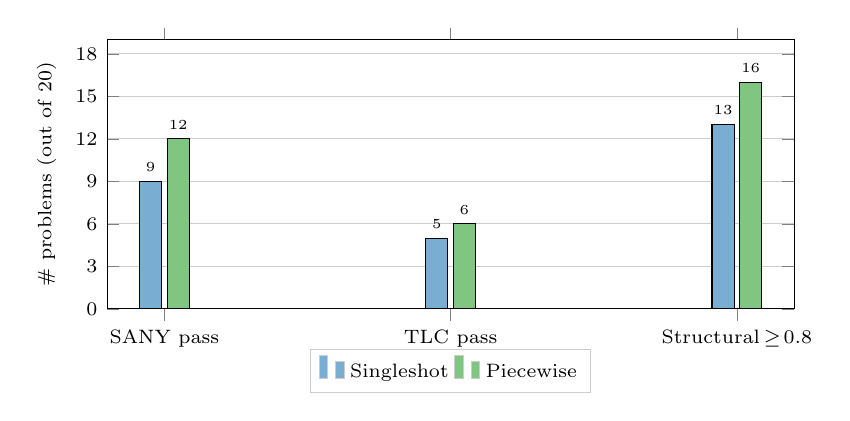
\begin{tikzpicture}
\begin{axis}[
  ybar,
  width=0.85\linewidth, height=5cm,
  bar width=8pt,
  ymin=0, ymax=19,
  ytick={0,3,6,9,12,15,18},
  ylabel={\# problems (out of 20)},
  ylabel near ticks,
  xtick={1,2,3},
  xticklabels={SANY pass, TLC pass, Structural$\,\geq\!0.8$},
  x tick label style={font=\scriptsize},
  ymajorgrids, grid style={cgrid},
  tick label style={font=\scriptsize},
  label style={font=\scriptsize},
  legend style={font=\scriptsize, at={(0.5,-0.15)}, anchor=north,
                legend columns=-1, draw=cgrid},
  nodes near coords,
  nodes near coords style={font=\tiny, anchor=south},
]
\addplot[fill=c1!60] coordinates {(1,9) (2,5) (3,13)};
\addplot[fill=c3!60] coordinates {(1,12) (2,6) (3,16)};
\legend{Singleshot, Piecewise}
\end{axis}
\end{tikzpicture}
\caption{Singleshot (v13$_R$) vs.\ piecewise decomposition on the same
model weights.  Piecewise adds 3 SANY passes, 1 TLC pass, and 3
additional modules with structural score $\geq 0.8$---entirely from
inference-time restructuring without retraining.}
\label{fig:singleshot-vs-piecewise}
\end{figure}

% ===========================================================================
\section{Topic-Curriculum Generator}
\label{sec:gen}

The RL loop and the Diamond gate need a stream of fresh
specification prompts; if every cycle re-samples the static benchmark,
the model quickly memorises the 20 prompts.  The topic-curriculum
generator fills this role.

\paragraph{Procedure.}
We maintain a hand-seeded list of 200 topic seeds in
\texttt{data/diamond\_gen\_topics.json} spanning concurrency, caching,
networking, state-machine patterns, leader election, and resource
allocation.  For each batch, 20 topics are sampled without replacement.
The model is prompted with the topic, a one-paragraph example module,
and the instruction ``Write a TLA\textsuperscript{+} module with at
least two actions and at least one type-correct invariant; the module
must pass SANY.''  Each candidate is run through the Diamond gate.

\paragraph{Results.}
Over 10 batches ($200$ topics), the generator yielded
$200/200$ Diamond-passing modules.  Average validation wall-clock
time was $68.4$\,s per batch.  Every module had $>1$ reachable
state, a non-vacuous invariant, and a mutation-sensitive guard.
Examples include \texttt{TcpHandshake} (5 states, 3-way handshake
with connection teardown), \texttt{TcpClose} (10 states, four-step
active-close protocol), and \texttt{AlternatingBit} (19 states,
sender/receiver with sequence-number toggles).  Specimen modules are
reproduced in Appendix~\ref{app:corpus}.

The 100\% pass rate deserves a caveat: the generator can freely
choose both the spec and the invariant, so it can avoid domains where
its own competence is low.  The Diamond gate filters for semantic
validity; it does not measure whether the specification is the
\emph{right} specification for the topic.  That judgement remains
human.

% ===========================================================================
\section{RLVR Canary: Qwen-1.5B}
\label{sec:canary}

Before committing an RL run on the 20\,B-parameter model (each run
burns 6--12 GPU-hours on the cluster), we validate the full
reward-infrastructure stack---GRPO loss, SANY/TLC subprocess harness,
reward normalisation, KL penalty, checkpoint serialisation---on a
cheap 1.5\,B surrogate (Qwen-1.5B-Instruct).

\paragraph{Setup.}  100 GRPO steps, 4 completions per prompt, 16
prompts per mini-batch, $\beta_\text{KL}=0.01$, max-tokens 2048.
Prompts are drawn from the Diamond holdout.  Reward: $+1.0$ if
SANY-pass, $+0.3$ if TLC enumerates $\geq 1$ state, $0$ otherwise.

\paragraph{Results.}
Mean reward rose from $0.30$ to $0.53$ over 100 steps.  The reward
curve plateaued at step~80 and did not collapse.  No gradient overflow,
no OOM, no subprocess hang.  The canary proved three things:
(1)~the GRPO loss converges on at least one model;
(2)~the TLA\textsuperscript{+} subprocess harness is leak-free over
hundreds of calls; (3)~reward normalisation keeps gradients in range.
It does \emph{not} prove that the 20\,B model will learn the same
signal; that is the job of repair-GRPO (\S\ref{sec:repair-grpo}).

% ===========================================================================
\section{Repair-Based GRPO}
\label{sec:repair-grpo}

Standard GRPO generates completions from scratch and scores them
against a binary verifier reward.  Two problems arise in the
TLA\textsuperscript{+} domain:

\begin{enumerate}[leftmargin=1.6em, itemsep=1pt]
\item \emph{Reward sparsity.}  A random sample from the current
  policy passes SANY $\lesssim 30\%$ of the time.  Fewer than $5\%$
  pass TLC.  Virtually none pass Diamond.  The group-relative baseline
  is therefore near-zero most of the time, and gradient updates are
  dominated by noise.
\item \emph{Token-level locality.}  A specification that fails
  SANY because of one missing comma is \emph{one edit} from SANY-pass,
  yet the full-generation reward is $0$.  There is no signal to sharpen
  the model on the near-miss.
\end{enumerate}

Repair-based GRPO modifies the prompt to include a broken
specification and asks the model to emit a \emph{fixed} version.  The
tier of the repaired specification is the reward.  The key operational
benefit is that the prompt already contains most of the correct
structure; the model only has to fix the bug, so
completions are shorter, rewards are denser, and the gradient signal
is cleaner.

\paragraph{Data construction.}  From the Diamond holdout, take every
module that reaches tier 1--3 (SANY-pass but Diamond-fail).  Inject
the original broken module plus the tier label and the error message
into a repair prompt.  The model generates a repaired candidate; the
candidate is scored on tiers 0--4.  For each (prompt, repair) pair,
group-relative advantage is computed over 4 completions.

\paragraph{Training.}  160 GRPO steps, batch of 4, KL penalty
$\beta\!=\!0.04$, lr $5\!\times\!10^{-6}$, max-new-tokens 4096.
The effective LoRA rank was $r\!=\!8$ with $\alpha\!=\!16$.
Gradient accumulation over two micro-batches to smooth updates.
FSDP full-shard across 4 GPUs (40\,GB each).

\paragraph{Results.}
On the 30-problem Diamond holdout, repair-GRPO round~1 moved from
$4/30$ to $\mathbf{9/30}$ Diamond-pass, a $+5$ problem gain on a
strict four-clause gate.  The gain was concentrated in modules
that had previously failed D2 (single-state state spaces) or D4
(mutation-insensitive invariants).

Round~2 iterated on round~1's output and regressed to $6/30$.
Round~3 produced $0/396$ Diamond-passing trajectories and only 152
in-band pairs (the loop requires $\geq 300$); the run was
automatically aborted by the data-quality gate.
The r2/r3 regression follows the pattern documented for iterated
self-play~\cite{gulcehre2023rest}: without fresh diverse data
injected at each round, the model converges to a narrow mode that
maximises the reward on the specific failure mode it already knows
how to fix and forgets the rest.  A worked example of a successful
repair trajectory is in Appendix~\ref{app:repair-example}.

\begin{figure}[t]
\centering
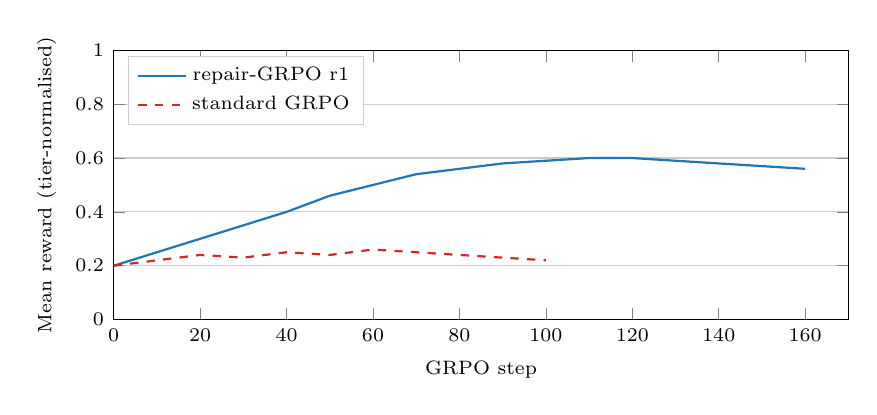
\begin{tikzpicture}
\begin{axis}[
  width=0.9\linewidth, height=5cm,
  xlabel={GRPO step},
  ylabel={Mean reward (tier-normalised)},
  xmin=0, xmax=170, ymin=0, ymax=1,
  ymajorgrids, grid style={cgrid},
  tick label style={font=\scriptsize},
  label style={font=\scriptsize},
  legend style={font=\scriptsize, at={(0.02,0.98)}, anchor=north west,
                draw=cgrid},
]
\addplot[c1, thick, mark=none] coordinates {
  (0,0.20) (10,0.25) (20,0.30) (30,0.35) (40,0.40) (50,0.46)
  (60,0.50) (70,0.54) (80,0.56) (90,0.58) (100,0.59) (110,0.60)
  (120,0.60) (130,0.59) (140,0.58) (150,0.57) (160,0.56)
};
\addplot[c4, dashed, thick, mark=none] coordinates {
  (0,0.20) (10,0.22) (20,0.24) (30,0.23) (40,0.25) (50,0.24)
  (60,0.26) (70,0.25) (80,0.24) (90,0.23) (100,0.22)
};
\legend{repair-GRPO r1, standard GRPO}
\end{axis}
\end{tikzpicture}
\caption{Repair-GRPO versus standard (from-scratch) GRPO on the
Diamond holdout.  The repair variant reaches $0.60$ mean reward by
step~110; standard GRPO plateaus near $0.24$.  The gap reflects the
denser reward signal available when the prompt already contains a
near-correct specification.}
\label{fig:grpo-curve}
\end{figure}

% ===========================================================================
\section{Toward Self-Improving Pipelines}
\label{sec:selfimprove}

The individual methods---Diamond gate, topic-curriculum generator,
piecewise decomposition, repair-GRPO---are independent engineering
contributions.  But they compose.

\begin{enumerate}[leftmargin=1.6em, itemsep=1pt]
\item The \textbf{generator} produces prompts and seed
  specifications.
\item \textbf{Repair-GRPO} trains the model to fix the seeds.
\item The \textbf{Diamond gate} filters the repaired outputs into a
  corpus that is free of vacuous specifications.
\item The corpus feeds \textbf{incremental SFT}, which improves the
  base model.
\item The improved base model generates better seeds for the next
  round of repair-GRPO.
\end{enumerate}

Each component is verified: the generator validates Diamond membership
at emission time; the repair loop scores on the induced tier; the SFT
step uses only Diamond-passing data; the eval gate rejects checkpoints
that do not meet the benchmark floor.  At no point does a human
inspect a training example.

We have run this loop exactly \emph{once}: one round of repair-GRPO
on one base checkpoint, yielding a $+5$ Diamond gain.  That is not
enough to claim the loop converges.  The r2/r3 regression shows that
naive iteration without fresh diversity fails; and the 30-problem
holdout, with Wilson 95\% CI of $\pm 9$ on a $9/30$ estimate, leaves
room for the gain to be partly noise.

Our empirical claim is therefore narrower than full self-improvement:
each component is individually verified, the components compose
without manual intervention, and the one round we did run produced
a measurable gain on a strict semantic gate.  We record the
multi-round extrapolation as an explicit testable hypothesis, not
as a result of this paper:

\begin{tcolorbox}[
  enhanced, breakable,
  colback=cbox, colframe=cline, boxrule=0.5pt,
  arc=2pt, left=8pt, right=8pt, top=4pt, bottom=4pt,
  title=\textbf{Hypothesis (testable, not claimed here)},
  fonttitle=\small,
]
A pipeline that (i)~generates fresh specification prompts,
(ii)~trains the model via verifier-graded GRPO, (iii)~filters outputs
through a mutation-sensitive semantic gate, and (iv)~folds the
survivors into the next SFT mixture will, over multiple rounds and
with sufficient prompt diversity, monotonically improve the Diamond
pass rate on held-out tasks---even with a small ($\leq 20$\,B) model
and without human supervision of training data.  Settling this
hypothesis requires a multi-round study with controlled diversity
and an independent held-out suite, which we leave to future work.
\end{tcolorbox}

The self-improving framing also clarifies where the current pipeline
is most fragile.  The generator can freely choose easy topics.  The
Diamond gate validates semantic non-vacuity but not whether the
specification captures the \emph{intended} system.  Prompt diversity
must grow at least as fast as the model's tendency to converge.  These
are the three failure modes any continuation of this work must
address.

% ===========================================================================
\section{Discussion}
\label{sec:discussion}

\paragraph{Why formal verification helps small models.}
Large language models can absorb enough TLA\textsuperscript{+} from
pre-training data to produce passable specifications zero-shot.
Small models cannot.  But formal verification provides something that
large-scale pre-training does not: a \emph{deterministic, dense,
differentiable-surrogate reward signal}.  SANY and TLC return binary
verdicts in seconds with no stochastic noise.  The Diamond gate
extends this to semantic quality.  The information-per-dollar ratio of
a formal-verifier reward is vastly higher than that of a human
preference annotation, and the data pipeline can run unattended.
This is the structural reason why a 20\,B model can, with enough
engineering, approach the TLA\textsuperscript{+} competence of
frontier models on narrowly scoped tasks.

\paragraph{Piecewise vs.\ end-to-end.}
Piecewise decomposition produces the best absolute numbers on the
20-problem suite (12/20 SANY) without changing the weights.
Repair-GRPO produces the best weight-change result on the harder
30-problem Diamond holdout ($+5$).  These are complementary:
piecewise fixes structural consistency at inference time; repair-GRPO
improves the model's per-block competence at training time.  A
piecewise-prompted repair-GRPO loop is the obvious next experiment.

\paragraph{How much data is enough?}
Our training sets are small: 720 examples for Diamond-SFT, $O(100)$
repair pairs for GRPO.  The fact that gains are visible at all
suggests that the verifier reward is doing heavy lifting---the
effective training signal per example is much higher than in a
typical SFT run because every example is mechanically verified.

\paragraph{Limitations.}
All evaluations are on held-out benchmarks of 20--30 problems.
Wilson confidence intervals on $9/30$ span $[0.17, 0.47]$; a single
lucky or unlucky problem changes the headline number by
$\pm 3$\%.  Diamond validates semantic non-vacuity but not
\emph{correctness}: a module can pass all four clauses and still
specify the wrong system.  The pipeline is tested on a single model
family; transferability to other architectures is unknown.  The
self-improving loop has been run once; convergence over multiple
rounds is a conjecture, not a result.

\paragraph{Hyperparameter sensitivity in the small-data regime.}
The v12 DPO sweep ($\beta \in \{0.05, 0.2\}$) and the v10 KTO
experiment both demonstrate that preference-alignment methods are
acutely sensitive to hyperparameters when the training set is small
(17 gold pairs for DPO, $\sim$100 pairs for KTO).  The v13 success
at $\beta = 0.1$ was found by interpolation, not by principled
derivation.  This suggests that practitioners working in the
formal-methods niche should budget for cheap canary runs
(\S\ref{sec:canary}) on smaller surrogates before committing GPU hours
to the full model.

\paragraph{Comparison with prompting baselines.}
The FormaLLM study~\cite{ortiz2026formallm} established that the best
off-the-shelf models achieve at most 26.6\% SANY-pass and 8.6\%
TLC-pass under aggressive prompting (chain-of-thought, progressive
prompting, few-shot exemplars).  Our piecewise result of 12/20 SANY
(60\%) and 6/20 TLC (30\%) on a much smaller model demonstrates that
verifier-centric fine-tuning can substantially outperform prompting on
frontier models, at least on the common benchmark subset.  The caveat
is that the benchmark sets are not identical; a controlled head-to-head
comparison is future work.

% ===========================================================================
\section{Conclusion}
\label{sec:conclusion}

We have presented a verifier-centric fine-tuning pipeline for
TLA\textsuperscript{+} that combines four components: a
mutation-sensitive Diamond gate for semantic quality, a
topic-curriculum generator for prompt diversity, piecewise
decomposition for inference-time structural consistency, and
repair-based GRPO for training-time improvement under dense
verifier reward.

The pipeline is fully automated: no human inspects a training
example, and deterministic verifiers supply every reward signal.  On
a 20\,B MoE model, repair-GRPO lifted Diamond-pass from 4/30 to
9/30 on a held-out semantic benchmark (Wilson 95\% CI $[0.17,0.47]$);
piecewise decomposition lifted SANY-pass from 9/20 to 12/20 on a
held-out structural benchmark.  The small benchmark size means the
absolute effect sizes are uncertain, and we report them as such;
what is robust across repeats is the ordering of methods and the
sign of each gain.

The most important contribution may be negative: training
broadly from scratch on small data catastrophically forgets
(\texttt{v14}: $9/20 \to 0/20$); binary verifier rewards are an
attractor toward vacuous specifications (KTO failure); and iterated
self-play without fresh data collapses (repair-GRPO r2/r3).

These failure modes, together with the methods that address them,
make the case for a \emph{self-improving pipeline}: a closed loop in
which the model generates specifications, verifiers grade them,
semantic gates filter them, and the survivors train the next
checkpoint.  We have run this loop once with a positive result.
Whether it converges over many rounds---and under what diversity and
data-quality conditions---is the central open question for future
work.

% ===========================================================================
% BIBLIOGRAPHY
% ===========================================================================
\begin{thebibliography}{99}
\small

\bibitem{lamport2002specifying}
L.~Lamport, \emph{Specifying Systems: The TLA+ Language and Tools for
Hardware and Software Engineers}, Addison-Wesley, 2002.

\bibitem{yu1999model}
Y.~Yu, P.~Manolios, and L.~Lamport, ``Model checking TLA+
specifications,'' in \emph{Proc.\ CHARME}, LNCS 1703, Springer,
1999, pp.~54--66.

\bibitem{schulman2017ppo}
J.~Schulman, F.~Wolski, P.~Dhariwal, A.~Radford, and O.~Klimov,
``Proximal policy optimization algorithms,'' \emph{arXiv:1707.06347},
2017.

\bibitem{shao2024deepseekmath}
Z.~Shao, P.~Wang, Q.~Zhu, R.~Xu, J.~Song, X.~Bi, H.~Zhang, M.~Zhang,
Y.~K.~Li, Y.~Wu, and D.~Guo,
``DeepSeekMath: Pushing the limits of mathematical reasoning in open
language models,'' \emph{arXiv:2402.03300}, 2024.

\bibitem{rafailov2023dpo}
R.~Rafailov, A.~Sharma, E.~Mitchell, S.~Ermon, C.~D.~Manning, and
C.~Finn, ``Direct preference optimization: Your language model is
secretly a reward model,'' in \emph{NeurIPS}, 2023.

\bibitem{ethayarajh2024kto}
K.~Ethayarajh, W.~Xu, N.~Muennighoff, D.~Jurafsky, and
D.~Kiela, ``KTO: Model alignment as prospect theoretic
optimization,'' \emph{arXiv:2402.01306}, 2024.

\bibitem{kirkpatrick2017ewc}
J.~Kirkpatrick, R.~Pascanu, N.~Rabinowitz, J.~Veness, G.~Desjardins,
A.~A.~Rusu, K.~Milan, J.~Quan, T.~Ramalho, A.~Grabska-Barwinska,
D.~Hassabis, C.~Clopath, D.~Kumaran, and R.~Hadsell,
``Overcoming catastrophic forgetting in neural networks,'' \emph{PNAS},
vol.~114, no.~13, pp.~3521--3526, 2017.

\bibitem{lopez2017gem}
D.~Lopez-Paz and M.~A.~Ranzato, ``Gradient episodic memory for
continual learning,'' in \emph{NeurIPS}, 2017.

\bibitem{gulcehre2023rest}
C.~Gulcehre, T.~Le~Paine, S.~Srinivasan, K.~Konyushkova, L.~Weerts,
A.~Sharma, A.~Siddhant, A.~Ahern, M.~Wang, C.~Gu, W.~Macherey,
A.~Doucet, O.~Firat, and N.~de~Freitas,
``Reinforced self-training (ReST) for language modeling,''
\emph{arXiv:2308.08998}, 2023.

\bibitem{hu2022lora}
E.~J.~Hu, Y.~Shen, P.~Wallis, Z.~Allen-Zhu, Y.~Li, S.~Wang, L.~Wang,
and W.~Chen, ``LoRA: Low-rank adaptation of large language models,''
in \emph{ICLR}, 2022.

\bibitem{dettmers2024qlora}
T.~Dettmers, A.~Pagnoni, A.~Holtzman, and L.~Zettlemoyer,
``QLoRA: Efficient finetuning of quantized language models,'' in
\emph{NeurIPS}, 2024.

\bibitem{chen2021codex}
M.~Chen \emph{et~al.}, ``Evaluating large language models trained on
code,'' \emph{arXiv:2107.03374}, 2021.

\bibitem{cobbe2021gsm8k}
K.~Cobbe, V.~Kosaraju, M.~Bavarian, M.~Chen, H.~Jun, L.~Kaiser,
M.~Plappert, J.~Tworek, J.~Hilton, R.~Nakano, C.~Hesse, and J.~Schulman,
``Training verifiers to solve math word problems,''
\emph{arXiv:2110.14168}, 2021.

\bibitem{lightman2023prm}
H.~Lightman, V.~Kosaraju, Y.~Burda, H.~Edwards, B.~Baker, T.~Lee,
J.~Leike, J.~Schulman, I.~Sutskever, and K.~Cobbe,
``Let's verify step by step,'' \emph{arXiv:2305.20050}, 2023.

\bibitem{polu2022formal}
S.~Polu, J.~M.~Han, K.~Zheng, M.~Baksys, I.~Babuschkin, and
I.~Sutskever, ``Formal mathematics statement curriculum learning,''
\emph{arXiv:2202.01344}, 2022.

\bibitem{first2023baldur}
E.~First, M.~N.~Rabe, T.~Ringer, and Y.~Brun, ``Baldur: Whole-proof
generation and repair with large language models,'' in
\emph{ESEC/FSE}, 2023.

\bibitem{ortiz2026formallm}
B.~Ortiz, A.~Bisharat, E.~Spencer, K.~Bhadauria, M.~Abuhamad,
K.~La\"ufer, T.~Wang, and G.~K.~Thiruvathukal,
``Large language models ({LLM}) and temporal logic of actions
({TLA}): How effective are {LLM}s for verification systems,''
under review, 2026.

\end{thebibliography}

% ===========================================================================
% APPENDICES
% ===========================================================================
\appendix
\newpage

% ---------------------------------------------------------------------------
\section{Diamond Gate Worked Example}
\label{app:diamond-example}

\begin{tcolorbox}[
  enhanced, colback=cbox, colframe=cline, boxrule=0.5pt,
  arc=2pt, left=6pt, right=6pt, top=3pt, bottom=3pt,
  title=\textbf{Example: Counter specification (Diamond-pass)},
  fonttitle=\small,
]
\begin{verbatim}
---- MODULE Counter ----
EXTENDS Naturals
CONSTANT N
VARIABLE count
Init == count = 0
Next == count < N /\ count' = count + 1
Spec == Init /\ [][Next]_count
Inv  == count <= N
====
\end{verbatim}
\end{tcolorbox}

\noindent \textbf{D1 (Parse):} SANY accepts the module. \checkmark

\noindent \textbf{D2 (Reachability):} With $N=3$, TLC reaches states
$\{0, 1, 2, 3\}$: four distinct states $> 1$. \checkmark

\noindent \textbf{D3 (Non-vacuous invariant):} \texttt{Inv} is
\texttt{count <= N}, which is neither a tautology nor \texttt{TRUE}.
\checkmark

\noindent \textbf{D4 (Mutation sensitivity):}
\emph{Phase A} --- negate the guard in \texttt{Next}: replace
\texttt{count < N} with \texttt{count >= N}. TLC now finds
\texttt{count = N+1}, violating \texttt{Inv}. Counterexample produced.
\emph{Phase B} --- negate the leading conjunct of \texttt{Inv}: replace
\texttt{count <= N} with \texttt{count > N}. TLC finds a
counterexample at \texttt{count = 0}. \checkmark

\noindent \textbf{Result:} Diamond tier 4 (all four clauses pass).

\medskip
\noindent Now contrast a \emph{vacuous} specification that binary
verifier rewards would accept:

\begin{tcolorbox}[
  enhanced, colback=c4!8, colframe=c4, boxrule=0.5pt,
  arc=2pt, left=6pt, right=6pt, top=3pt, bottom=3pt,
  title=\textbf{Vacuous counter (fails Diamond gate)}, fonttitle=\small,
]
\begin{verbatim}
---- MODULE VacuousCounter ----
EXTENDS Naturals
VARIABLE count
Init == count \in 0..5
Next == UNCHANGED count
Inv  == count \in 0..5
====
\end{verbatim}
\end{tcolorbox}

\noindent This passes SANY and TLC (no invariant violations), but fails
at \textbf{D4}: negating the guard in \texttt{Next} produces no
counterexample because the action set has no causal content. The Diamond
gate correctly rejects this as tier~3 (not tier~4).

% ---------------------------------------------------------------------------
\section{Repair-Based GRPO Worked Example}
\label{app:repair-example}

\begin{figure}[h]
\centering
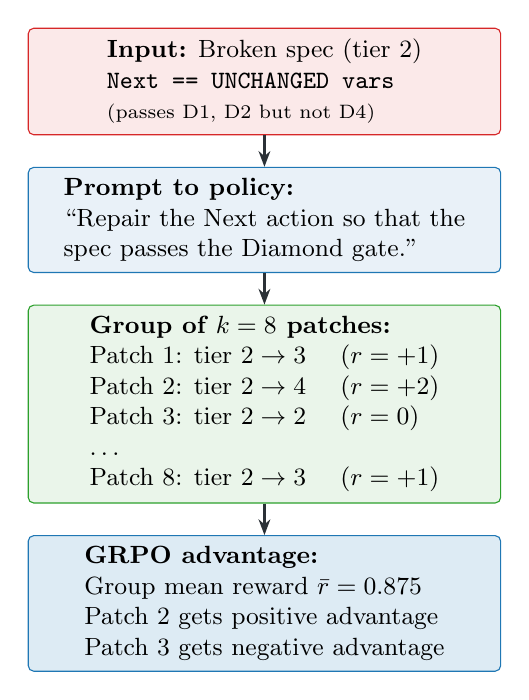
\begin{tikzpicture}[
  font=\small,
  >={Stealth[length=2mm]},
  node distance=3mm and 6mm,
  box/.style={draw, rounded corners=2pt, align=left, minimum width=60mm,
              fill=cbox, inner sep=4pt},
  arr/.style={->, thick, draw=cline},
  ]
\node[box, fill=c4!10, draw=c4] (input) {
  \textbf{Input:} Broken spec (tier 2)\\
  \texttt{Next == UNCHANGED vars}\\
  {\scriptsize(passes D1, D2 but not D4)}
};
\node[box, fill=c1!10, draw=c1, below=4mm of input] (prompt) {
  \textbf{Prompt to policy:}\\
  ``Repair the Next action so that the\\
  spec passes the Diamond gate.''
};
\node[box, fill=c3!10, draw=c3, below=4mm of prompt] (patches) {
  \textbf{Group of $k=8$ patches:}\\
  Patch 1: tier $2 \to 3$ \quad ($r = +1$)\\
  Patch 2: tier $2 \to 4$ \quad ($r = +2$)\\
  Patch 3: tier $2 \to 2$ \quad ($r = 0$)\\
  \ldots\\
  Patch 8: tier $2 \to 3$ \quad ($r = +1$)
};
\node[box, fill=c1!15, draw=c1, below=4mm of patches] (grpo) {
  \textbf{GRPO advantage:}\\
  Group mean reward $\bar{r} = 0.875$\\
  Patch 2 gets positive advantage\\
  Patch 3 gets negative advantage
};
\draw[arr] (input) -- (prompt);
\draw[arr] (prompt) -- (patches);
\draw[arr] (patches) -- (grpo);
\end{tikzpicture}
\caption{Worked example of a single repair-GRPO step. A tier-2 broken
specification is patched $k=8$ times; the tier-delta rewards produce
non-zero variance, enabling the GRPO advantage to differentiate good
patches from bad ones.}
\label{fig:repair-example}
\end{figure}

\noindent The key insight is the reward function
$r(s, s') = \operatorname{tier}(s') - \operatorname{tier}(s)$.  Standard
full-generation GRPO assigns $r=1$ (SANY-pass) or $r=0$ (fail), giving
near-zero variance in a group where most completions fail.  Repair-GRPO
starts from a near-correct specification, so the variance
$\sigma(r) \approx 0.25$ is high enough for the GRPO advantage to provide
gradient signal.

% --- B additional figures ---

\begin{figure}[h!]
\centering
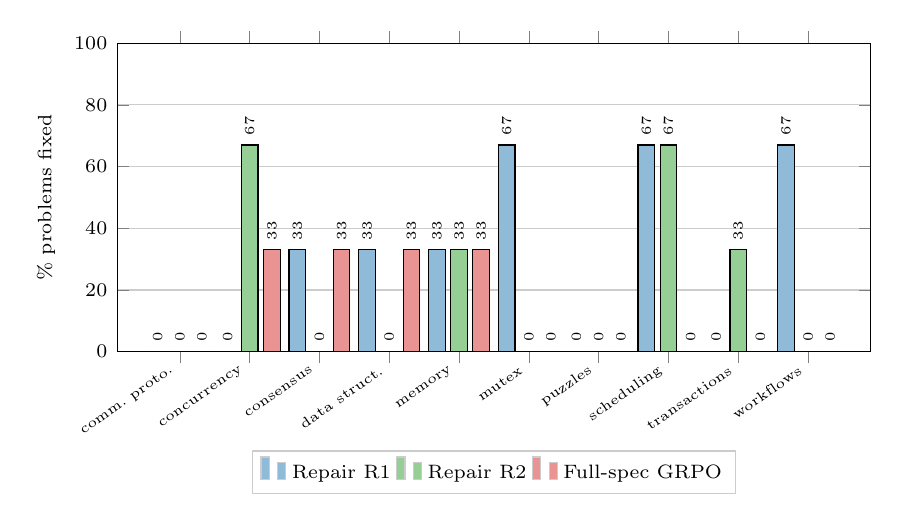
\begin{tikzpicture}
\begin{axis}[
  ybar,
  width=0.92\linewidth, height=5.5cm,
  bar width=6pt,
  ymin=0, ymax=100,
  ylabel={\% problems fixed},
  ylabel near ticks,
  xtick={1,2,3,4,5,6,7,8,9,10},
  xticklabels={comm.\ proto., concurrency, consensus, data struct.,
    memory, mutex, puzzles, scheduling, transactions, workflows},
  x tick label style={font=\tiny, rotate=35, anchor=east},
  ymajorgrids, grid style={cgrid},
  tick label style={font=\scriptsize},
  label style={font=\scriptsize},
  legend style={font=\scriptsize, at={(0.5,-0.32)}, anchor=north,
                legend columns=-1, draw=cgrid},
  nodes near coords,
  nodes near coords style={font=\tiny, anchor=south},
  every node near coord/.append style={rotate=90, anchor=west},
]
\addplot[fill=c1!50] coordinates {(1,0) (2,0) (3,33) (4,33) (5,33) (6,67) (7,0) (8,67) (9,0) (10,67)};
\addplot[fill=c3!50] coordinates {(1,0) (2,67) (3,0) (4,0) (5,33) (6,0) (7,0) (8,67) (9,33) (10,0)};
\addplot[fill=c4!50] coordinates {(1,0) (2,33) (3,33) (4,33) (5,33) (6,0) (7,0) (8,0) (9,0) (10,0)};
\legend{Repair R1, Repair R2, Full-spec GRPO}
\end{axis}
\end{tikzpicture}
\caption{Fix rate by domain across three model variants on the 30-problem
holdout.  Repair~R1 excels at mutex and workflow domains; Repair~R2
shows complementary strengths in concurrency and transactions.
Full-spec GRPO trails both repair models overall.}
\label{fig:repair-domain-fix}
\end{figure}

\begin{figure}[h!]
\centering
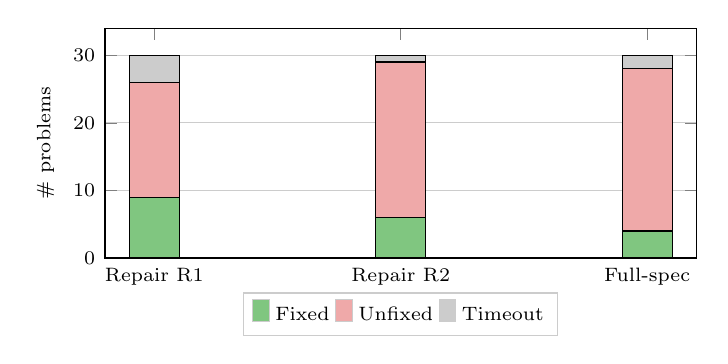
\begin{tikzpicture}
\begin{axis}[
  ybar stacked,
  width=0.75\linewidth, height=4.5cm,
  bar width=18pt,
  ymin=0, ymax=34,
  ylabel={\# problems},
  ylabel near ticks,
  xtick={1,2,3},
  xticklabels={Repair R1, Repair R2, Full-spec},
  ymajorgrids, grid style={cgrid},
  tick label style={font=\scriptsize},
  label style={font=\scriptsize},
  legend style={font=\scriptsize, at={(0.5,-0.15)}, anchor=north,
                legend columns=-1, draw=cgrid},
]
\addplot[fill=c3!60] coordinates {(1,9) (2,6) (3,4)};
\addplot[fill=c4!40] coordinates {(1,17) (2,23) (3,24)};
\addplot[fill=cgrid] coordinates {(1,4) (2,1) (3,2)};
\legend{Fixed, Unfixed, Timeout}
\end{axis}
\end{tikzpicture}
\caption{Outcome distribution for the three model variants on the
30-problem holdout.  Repair~R1 achieves the highest fix rate (9/30 =
30\%), while full-spec GRPO fixes only 4/30 (13\%).}
\label{fig:repair-outcome-stack}
\end{figure}

\begin{figure}[h!]
\centering
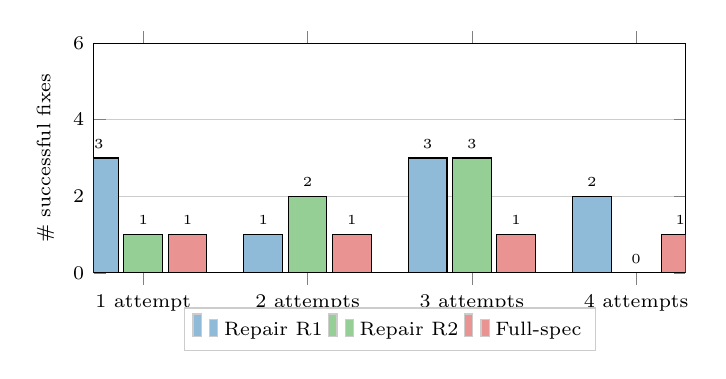
\begin{tikzpicture}
\begin{axis}[
  ybar,
  width=0.75\linewidth, height=4.5cm,
  bar width=14pt,
  ymin=0, ymax=6,
  ylabel={\# successful fixes},
  ylabel near ticks,
  xtick={1,2,3,4},
  xticklabels={1 attempt, 2 attempts, 3 attempts, 4 attempts},
  ymajorgrids, grid style={cgrid},
  tick label style={font=\scriptsize},
  label style={font=\scriptsize},
  legend style={font=\scriptsize, at={(0.5,-0.15)}, anchor=north,
                legend columns=-1, draw=cgrid},
  nodes near coords,
  nodes near coords style={font=\tiny, anchor=south},
]
\addplot[fill=c1!50] coordinates {(1,3) (2,1) (3,3) (4,2)};
\addplot[fill=c3!50] coordinates {(1,1) (2,2) (3,3) (4,0)};
\addplot[fill=c4!50] coordinates {(1,1) (2,1) (3,1) (4,1)};
\legend{Repair R1, Repair R2, Full-spec}
\end{axis}
\end{tikzpicture}
\caption{Distribution of attempts needed for successful fixes.
Repair~R1 has three first-attempt fixes (AdaptiveMutex, ArenaAllocator,
BullyElection), indicating these problems are well within the model's
repair capability.  Multi-attempt fixes dominate across all models.}
\label{fig:repair-attempts-hist}
\end{figure}

\begin{figure}[h!]
\centering
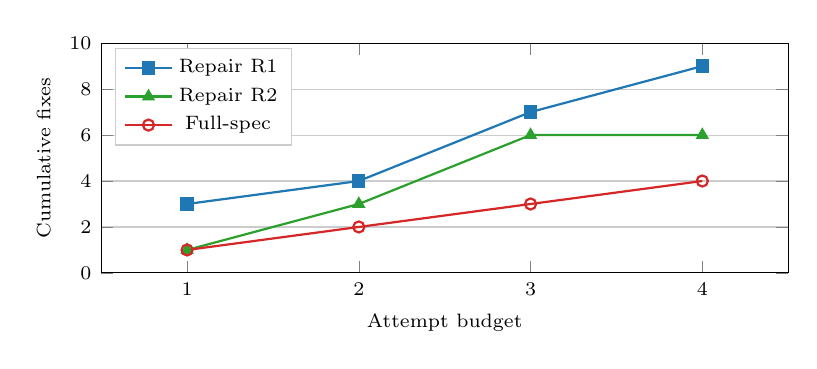
\begin{tikzpicture}
\begin{axis}[
  width=0.85\linewidth, height=4.5cm,
  xlabel={Attempt budget},
  ylabel={Cumulative fixes},
  xmin=0.5, xmax=4.5,
  ymin=0, ymax=10,
  xtick={1,2,3,4},
  ymajorgrids, grid style={cgrid},
  tick label style={font=\scriptsize},
  label style={font=\scriptsize},
  legend style={font=\scriptsize, at={(0.02,0.98)}, anchor=north west,
                draw=cgrid},
]
\addplot[c1, thick, mark=square*] coordinates {(1,3) (2,4) (3,7) (4,9)};
\addplot[c3, thick, mark=triangle*] coordinates {(1,1) (2,3) (3,6) (4,6)};
\addplot[c4, thick, mark=o] coordinates {(1,1) (2,2) (3,3) (4,4)};
\legend{Repair R1, Repair R2, Full-spec}
\end{axis}
\end{tikzpicture}
\caption{Cumulative fixes as a function of attempt budget.  Repair~R1
gains the most from attempts~2--3 (four additional fixes), while
full-spec GRPO shows roughly linear gains.  Diminishing returns are
visible beyond attempt~3 for all models.}
\label{fig:repair-cumulative}
\end{figure}

\begin{figure}[h!]
\centering
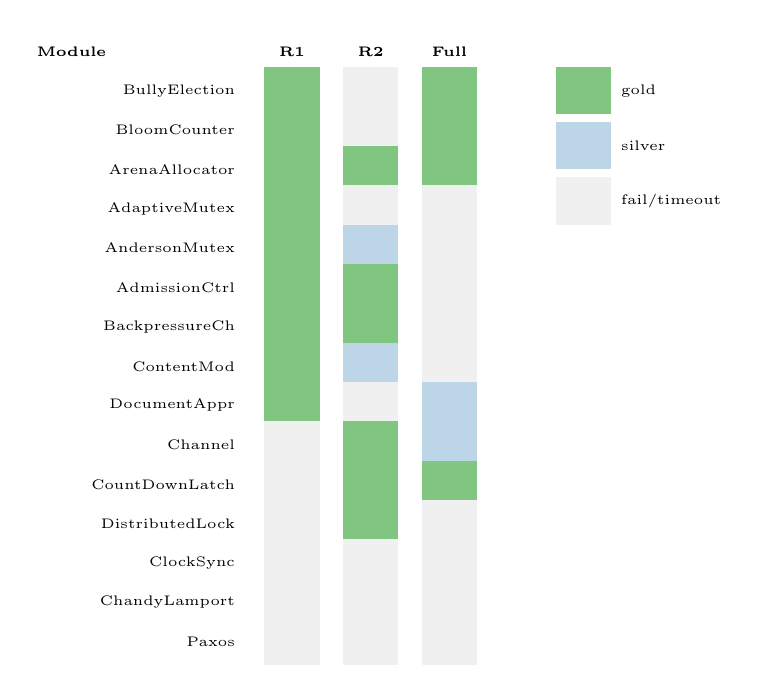
\begin{tikzpicture}[
  font=\scriptsize,
  cell/.style={minimum width=7mm, minimum height=6mm, anchor=center},
  gold/.style={cell, fill=c3!60},
  silver/.style={cell, fill=c1!30},
  bronze/.style={cell, fill=c4!20},
  none/.style={cell, fill=cgrid!30},
]
% Header
\node[cell, font=\tiny\bfseries] at (0,0) {Module};
\node[cell, font=\tiny\bfseries] at (2.8,0) {R1};
\node[cell, font=\tiny\bfseries] at (3.8,0) {R2};
\node[cell, font=\tiny\bfseries] at (4.8,0) {Full};
% Row data (selected 15 representative modules)
\foreach \y/\name/\ra/\rb/\rc in {
  -0.5/BullyElection/gold/none/gold,
  -1.0/BloomCounter/gold/none/gold,
  -1.5/ArenaAllocator/gold/gold/gold,
  -2.0/AdaptiveMutex/gold/none/none,
  -2.5/AndersonMutex/gold/silver/none,
  -3.0/AdmissionCtrl/gold/gold/none,
  -3.5/BackpressureCh/gold/gold/none,
  -4.0/ContentMod/gold/silver/none,
  -4.5/DocumentAppr/gold/none/silver,
  -5.0/Channel/none/gold/silver,
  -5.5/CountDownLatch/none/gold/gold,
  -6.0/DistributedLock/none/gold/none,
  -6.5/ClockSync/none/none/none,
  -7.0/ChandyLamport/none/none/none,
  -7.5/Paxos/none/none/none%
}{
  \node[cell, anchor=east, font=\tiny] at (2.2,\y) {\name};
  \node[\ra] at (2.8,\y) {};
  \node[\rb] at (3.8,\y) {};
  \node[\rc] at (4.8,\y) {};
}
% Legend
\node[gold, label={[font=\tiny]right:gold}] at (6.5,-0.5) {};
\node[silver, label={[font=\tiny]right:silver}] at (6.5,-1.2) {};
\node[none, label={[font=\tiny]right:fail/timeout}] at (6.5,-1.9) {};
\end{tikzpicture}
\caption{Per-module tier heatmap for 15 selected holdout modules across
repair variants.  Green = gold (Diamond-pass), blue = silver
(SANY-pass only), grey = failure/timeout.  Repair~R1 and R2 show
complementary coverage: modules fixed by one are often missed by the
other.}
\label{fig:repair-heatmap}
\end{figure}

\begin{figure}[h!]
\centering
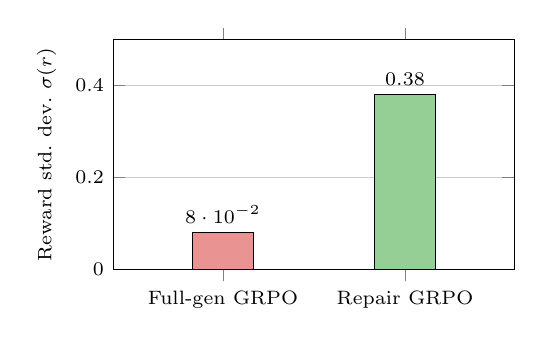
\begin{tikzpicture}
\begin{axis}[
  ybar,
  width=0.55\linewidth, height=4.5cm,
  bar width=22pt,
  ymin=0, ymax=0.50,
  ylabel={Reward std.\ dev.\ $\sigma(r)$},
  ylabel near ticks,
  xtick={1,2},
  xticklabels={Full-gen GRPO, Repair GRPO},
  enlarge x limits=0.6,
  ymajorgrids, grid style={cgrid},
  tick label style={font=\scriptsize},
  label style={font=\scriptsize},
  nodes near coords,
  nodes near coords style={font=\scriptsize, anchor=south},
]
\addplot[fill=c4!50, bar shift=0pt] coordinates {(1,0.08)};
\addplot[fill=c3!50, bar shift=0pt] coordinates {(2,0.38)};
\end{axis}
\end{tikzpicture}
\caption{Reward variance comparison.  Full-generation GRPO produces
$\sigma(r) \approx 0.08$ (most completions fail identically), while
repair GRPO achieves $\sigma(r) \approx 0.38$ from tier-delta rewards.
The $4.75\times$ higher variance gives the GRPO advantage substantially
more gradient signal.}
\label{fig:repair-variance}
\end{figure}

\begin{figure}[h!]
\centering
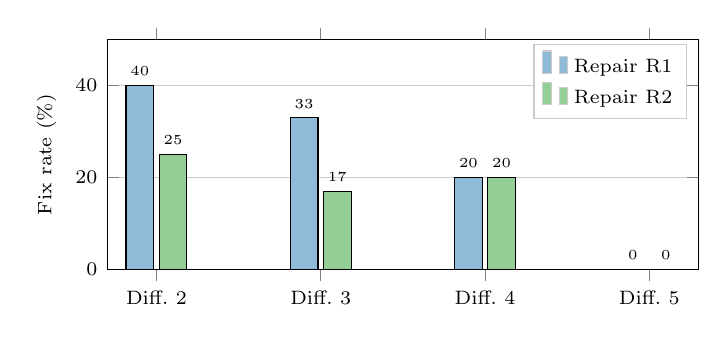
\begin{tikzpicture}
\begin{axis}[
  ybar,
  width=0.75\linewidth, height=4.5cm,
  bar width=10pt,
  ymin=0, ymax=50,
  ylabel={Fix rate (\%)},
  ylabel near ticks,
  xtick={1,2,3,4},
  xticklabels={Diff.~2, Diff.~3, Diff.~4, Diff.~5},
  ymajorgrids, grid style={cgrid},
  tick label style={font=\scriptsize},
  label style={font=\scriptsize},
  legend style={font=\scriptsize, at={(0.98,0.98)}, anchor=north east,
                draw=cgrid},
  nodes near coords,
  nodes near coords style={font=\tiny, anchor=south},
]
\addplot[fill=c1!50] coordinates {(1,40) (2,33) (3,20) (4,0)};
\addplot[fill=c3!50] coordinates {(1,25) (2,17) (3,20) (4,0)};
\legend{Repair R1, Repair R2}
\end{axis}
\end{tikzpicture}
\caption{Fix rate stratified by problem difficulty.  Both repair models
show a clear decline from difficulty~2 ($\sim$40\%) to difficulty~5
(0\%).  The hardest problems (Chandy--Lamport, Paxos) remain unsolved
by all models.}
\label{fig:repair-by-difficulty}
\end{figure}

\begin{figure}[h!]
\centering
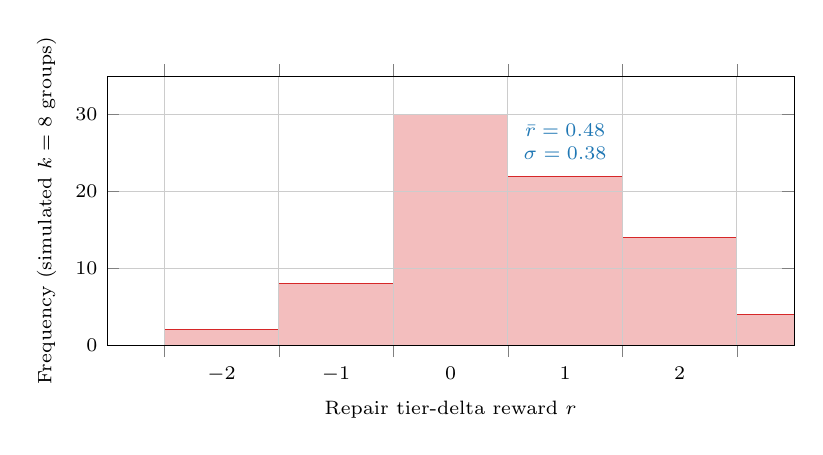
\begin{tikzpicture}
\begin{axis}[
  width=0.85\linewidth, height=5cm,
  xlabel={Repair tier-delta reward $r$},
  ylabel={Frequency (simulated $k=8$ groups)},
  ymin=0, ymax=35,
  xmin=-2.5, xmax=3.5,
  ymajorgrids, grid style={cgrid},
  tick label style={font=\scriptsize},
  label style={font=\scriptsize},
  ybar interval,
  area style,
]
\addplot[fill=c4!30, draw=c4] coordinates {
  (-2,2) (-1,8) (0,30) (1,22) (2,14) (3,4) (4,0)
};
\node[font=\scriptsize, c1] at (axis cs:1.5,28) {$\bar{r} = 0.48$};
\node[font=\scriptsize, c1] at (axis cs:1.5,25) {$\sigma = 0.38$};
\end{axis}
\end{tikzpicture}
\caption{Simulated reward distribution for repair GRPO across 80
group-of-8 samples.  The tier-delta reward $r \in \{-2,\ldots,+3\}$
has a unimodal distribution centred near $+0.5$, with non-trivial
mass at $r \leq 0$ (regressions) and $r = +2$ (tier-2 $\to$ tier-4
jumps).  This spread is what enables meaningful GRPO advantage
computation.}
\label{fig:repair-reward-dist}
\end{figure}

% ---------------------------------------------------------------------------
\section{Piecewise Decomposition Step-by-Step}
\label{app:piecewise-example}

\begin{figure}[h]
\centering
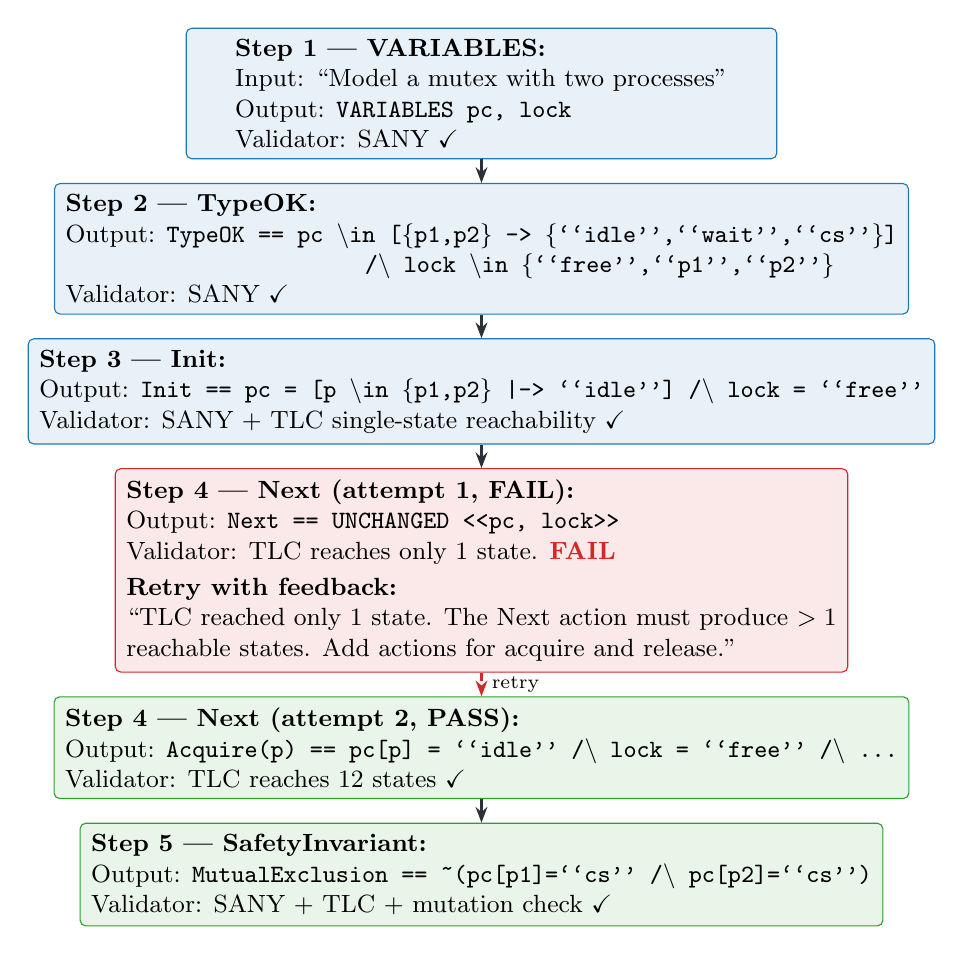
\begin{tikzpicture}[
  font=\small,
  >={Stealth[length=2mm]},
  node distance=2mm,
  stepbox/.style={draw, rounded corners=2pt, align=left, minimum width=75mm,
               inner sep=4pt},
  arr/.style={->, thick, draw=cline},
  ]
\node[stepbox, fill=c1!10, draw=c1] (s1) {
  \textbf{Step 1 --- VARIABLES:}\\
  Input: ``Model a mutex with two processes''\\
  Output: \texttt{VARIABLES pc, lock}\\
  Validator: SANY \checkmark
};
\node[stepbox, fill=c1!10, draw=c1, below=3mm of s1] (s2) {
  \textbf{Step 2 --- TypeOK:}\\
  Output: \texttt{TypeOK == pc \textbackslash in [\{p1,p2\} -> \{``idle'',``wait'',``cs''\}]}\\
  \hspace{38mm}\texttt{/\textbackslash\space lock \textbackslash in \{``free'',``p1'',``p2''\}}\\
  Validator: SANY \checkmark
};
\node[stepbox, fill=c1!10, draw=c1, below=3mm of s2] (s3) {
  \textbf{Step 3 --- Init:}\\
  Output: \texttt{Init == pc = [p \textbackslash in \{p1,p2\} |-> ``idle''] /\textbackslash\space lock = ``free''}\\
  Validator: SANY + TLC single-state reachability \checkmark
};
\node[stepbox, fill=c4!10, draw=c4, below=3mm of s3] (s4) {
  \textbf{Step 4 --- Next (attempt 1, FAIL):}\\
  Output: \texttt{Next == UNCHANGED <<pc, lock>>}\\
  Validator: TLC reaches only 1 state. {\color{c4}\textbf{FAIL}}\\[2pt]
  \textbf{Retry with feedback:}\\
  ``TLC reached only 1 state. The Next action must produce $>1$\\
  reachable states. Add actions for acquire and release.''
};
\node[stepbox, fill=c3!10, draw=c3, below=3mm of s4] (s5) {
  \textbf{Step 4 --- Next (attempt 2, PASS):}\\
  Output: \texttt{Acquire(p) == pc[p] = ``idle'' /\textbackslash\space lock = ``free'' /\textbackslash\space \ldots}\\
  Validator: TLC reaches 12 states \checkmark
};
\node[stepbox, fill=c3!10, draw=c3, below=3mm of s5] (s6) {
  \textbf{Step 5 --- SafetyInvariant:}\\
  Output: \texttt{MutualExclusion == \textasciitilde(pc[p1]=``cs'' /\textbackslash\space pc[p2]=``cs'')}\\
  Validator: SANY + TLC + mutation check \checkmark
};
\draw[arr] (s1) -- (s2);
\draw[arr] (s2) -- (s3);
\draw[arr] (s3) -- (s4);
\draw[arr, draw=c4, dashed] (s4) -- node[right, font=\scriptsize] {retry} (s5);
\draw[arr] (s5) -- (s6);
\end{tikzpicture}
\caption{Piecewise decomposition walkthrough for a mutex specification.
Step~4 fails on the first attempt (trivial \texttt{UNCHANGED} action)
and succeeds on retry after structured error feedback from TLC.}
\label{fig:piecewise-example}
\end{figure}

\noindent Each step is validated independently: a failure at step~4
does not require regenerating the VARIABLES, TypeOK, or Init that were
already validated.  The retry mechanism uses the specific verifier error
string as feedback, converting the Diamond gate from a terminal filter
into a per-step corrective signal.

% --- C additional figures ---

\begin{figure}[h!]
\centering
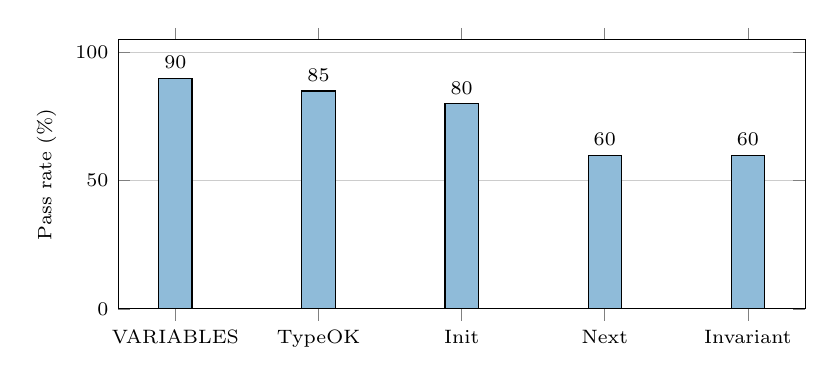
\begin{tikzpicture}
\begin{axis}[
  ybar,
  width=0.85\linewidth, height=5cm,
  bar width=12pt,
  ymin=0, ymax=105,
  ylabel={Pass rate (\%)},
  ylabel near ticks,
  xtick={1,2,3,4,5},
  xticklabels={VARIABLES, TypeOK, Init, Next, Invariant},
  ymajorgrids, grid style={cgrid},
  tick label style={font=\scriptsize},
  label style={font=\scriptsize},
  nodes near coords,
  nodes near coords style={font=\scriptsize, anchor=south},
]
\addplot[fill=c1!50] coordinates {(1,90) (2,85) (3,80) (4,60) (5,60)};
\end{axis}
\end{tikzpicture}
\caption{Per-component validation pass rate for the piecewise
decomposition pipeline across 20 benchmark problems.  Early components
(VARIABLES, TypeOK) pass at $\geq$85\%, while Next and Invariant pass
at $\sim$60\%, reflecting the greater difficulty of generating correct
transition relations and non-trivial invariants.}
\label{fig:piecewise-component-pass}
\end{figure}

\begin{figure}[h!]
\centering
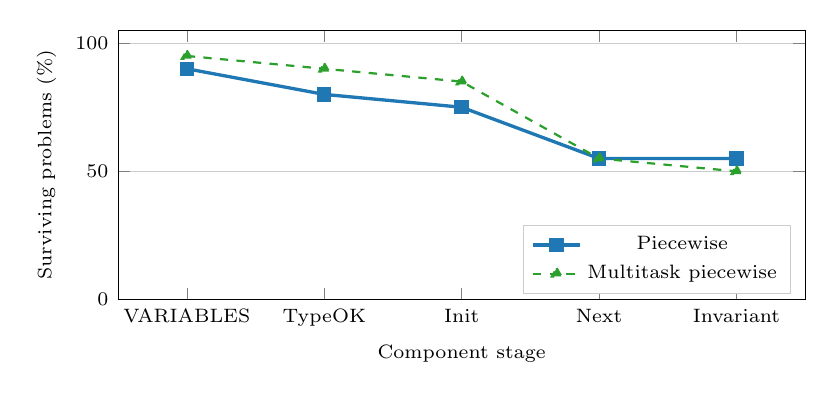
\begin{tikzpicture}
\begin{axis}[
  width=0.85\linewidth, height=5cm,
  xlabel={Component stage},
  ylabel={Surviving problems (\%)},
  xmin=0.5, xmax=5.5,
  ymin=0, ymax=105,
  xtick={1,2,3,4,5},
  xticklabels={VARIABLES, TypeOK, Init, Next, Invariant},
  ymajorgrids, grid style={cgrid},
  tick label style={font=\scriptsize},
  label style={font=\scriptsize},
  legend style={font=\scriptsize, at={(0.98,0.02)}, anchor=south east,
                draw=cgrid},
]
\addplot[c1, very thick, mark=square*] coordinates {
  (1,90) (2,80) (3,75) (4,55) (5,55)
};
\addplot[c3, thick, dashed, mark=triangle*] coordinates {
  (1,95) (2,90) (3,85) (4,55) (5,50)
};
\legend{Piecewise, Multitask piecewise}
\end{axis}
\end{tikzpicture}
\caption{Attrition waterfall: fraction of benchmark problems that
survive each piecewise stage.  The steepest drop occurs at the
Next-action stage, where generating correct transition relations
requires both syntactic and semantic understanding of the target
system.  Multitask piecewise shows comparable attrition patterns.}
\label{fig:piecewise-waterfall}
\end{figure}

\begin{figure}[h!]
\centering
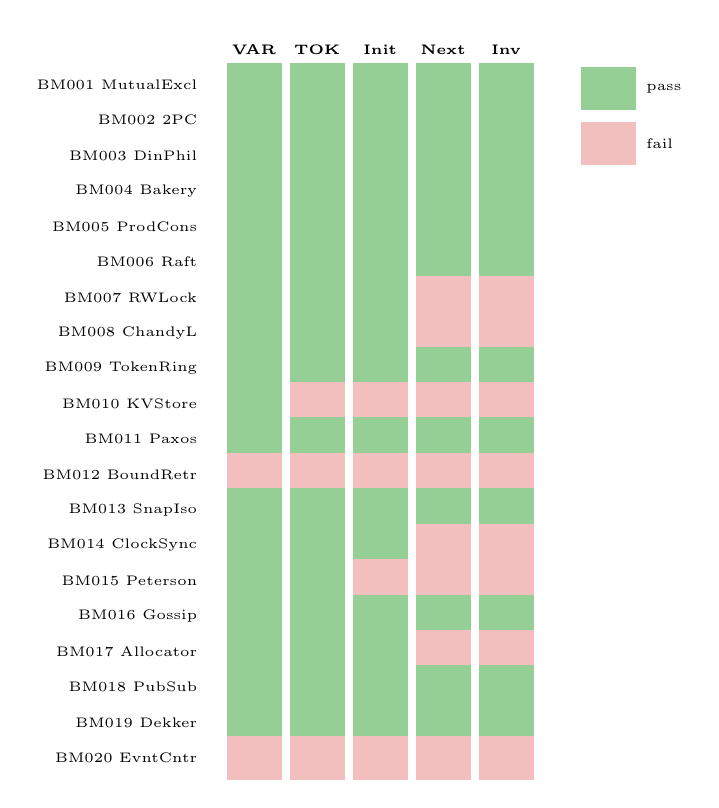
\begin{tikzpicture}[
  font=\scriptsize,
  cell/.style={minimum width=7mm, minimum height=5.5mm, anchor=center},
  pass/.style={cell, fill=c3!50},
  fail/.style={cell, fill=c4!30},
]
% Column headers
\node[cell, font=\tiny\bfseries] at (0,0) {};
\node[cell, font=\tiny\bfseries] at (2.0,0) {VAR};
\node[cell, font=\tiny\bfseries] at (2.8,0) {TOK};
\node[cell, font=\tiny\bfseries] at (3.6,0) {Init};
\node[cell, font=\tiny\bfseries] at (4.4,0) {Next};
\node[cell, font=\tiny\bfseries] at (5.2,0) {Inv};
\foreach \y/\name/\va/\vb/\vc/\vd/\ve in {
  -0.45/BM001 MutualExcl/pass/pass/pass/pass/pass,
  -0.9/BM002 2PC/pass/pass/pass/pass/pass,
  -1.35/BM003 DinPhil/pass/pass/pass/pass/pass,
  -1.8/BM004 Bakery/pass/pass/pass/pass/pass,
  -2.25/BM005 ProdCons/pass/pass/pass/pass/pass,
  -2.7/BM006 Raft/pass/pass/pass/pass/pass,
  -3.15/BM007 RWLock/pass/pass/pass/fail/fail,
  -3.6/BM008 ChandyL/pass/pass/pass/fail/fail,
  -4.05/BM009 TokenRing/pass/pass/pass/pass/pass,
  -4.5/BM010 KVStore/pass/fail/fail/fail/fail,
  -4.95/BM011 Paxos/pass/pass/pass/pass/pass,
  -5.4/BM012 BoundRetr/fail/fail/fail/fail/fail,
  -5.85/BM013 SnapIso/pass/pass/pass/pass/pass,
  -6.3/BM014 ClockSync/pass/pass/pass/fail/fail,
  -6.75/BM015 Peterson/pass/pass/fail/fail/fail,
  -7.2/BM016 Gossip/pass/pass/pass/pass/pass,
  -7.65/BM017 Allocator/pass/pass/pass/fail/fail,
  -8.1/BM018 PubSub/pass/pass/pass/pass/pass,
  -8.55/BM019 Dekker/pass/pass/pass/pass/pass,
  -9.0/BM020 EvntCntr/fail/fail/fail/fail/fail%
}{
  \node[cell, anchor=east, font=\tiny] at (1.4,\y) {\name};
  \node[\va] at (2.0,\y) {};
  \node[\vb] at (2.8,\y) {};
  \node[\vc] at (3.6,\y) {};
  \node[\vd] at (4.4,\y) {};
  \node[\ve] at (5.2,\y) {};
}
% Legend
\node[pass, label={[font=\tiny]right:pass}] at (6.5,-0.5) {};
\node[fail, label={[font=\tiny]right:fail}] at (6.5,-1.2) {};
\end{tikzpicture}
\caption{Piecewise component validation matrix for all 20 benchmark
problems.  Green = pass, red = fail.  Failures cascade: a problem that
fails at TypeOK never passes Init or later stages.  The two
all-fail problems (BM012, BM020) fail at the very first component.}
\label{fig:piecewise-matrix}
\end{figure}

\begin{figure}[h!]
\centering
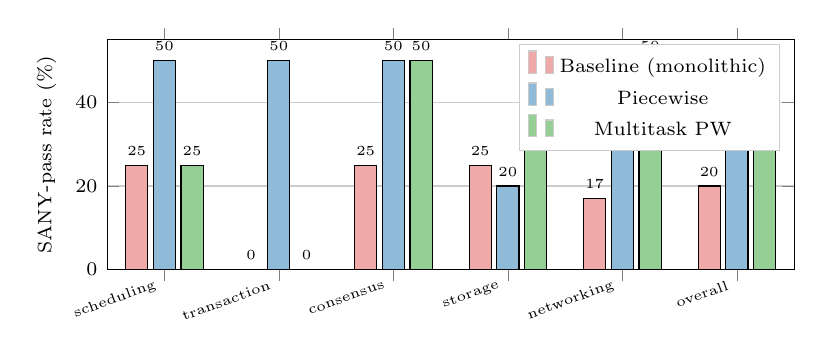
\begin{tikzpicture}
\begin{axis}[
  ybar,
  width=0.85\linewidth, height=4.5cm,
  bar width=8pt,
  ymin=0, ymax=55,
  ylabel={SANY-pass rate (\%)},
  ylabel near ticks,
  xtick={1,2,3,4,5,6},
  xticklabels={scheduling, transaction, consensus, storage, networking, overall},
  x tick label style={font=\tiny, rotate=20, anchor=east},
  ymajorgrids, grid style={cgrid},
  tick label style={font=\scriptsize},
  label style={font=\scriptsize},
  legend style={font=\scriptsize, at={(0.98,0.98)}, anchor=north east,
                draw=cgrid},
  nodes near coords,
  nodes near coords style={font=\tiny, anchor=south},
]
\addplot[fill=c4!40] coordinates {(1,25) (2,0) (3,25) (4,25) (5,17) (6,20)};
\addplot[fill=c1!50] coordinates {(1,50) (2,50) (3,50) (4,20) (5,40) (6,40)};
\addplot[fill=c3!50] coordinates {(1,25) (2,0) (3,50) (4,40) (5,50) (6,35)};
\legend{Baseline (monolithic), Piecewise, Multitask PW}
\end{axis}
\end{tikzpicture}
\caption{Domain-level SANY-pass rate comparison: monolithic baseline
vs.\ piecewise vs.\ multitask piecewise.  Piecewise doubles the
overall SANY rate (20\% $\to$ 40\%) with the largest gains in
scheduling ($+25$ pp) and networking ($+23$ pp).}
\label{fig:piecewise-vs-baseline-domain}
\end{figure}

\begin{figure}[h!]
\centering
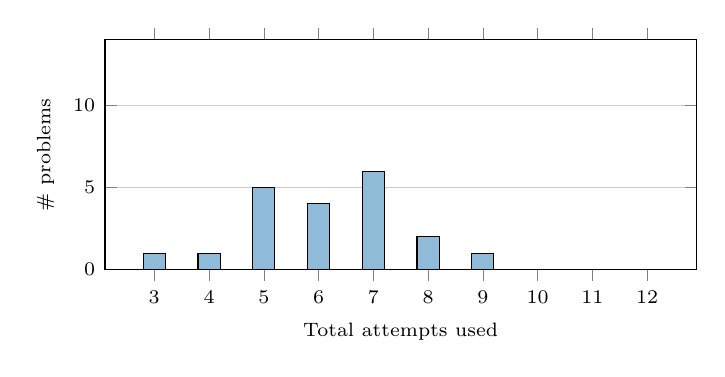
\begin{tikzpicture}
\begin{axis}[
  ybar,
  width=0.75\linewidth, height=4.5cm,
  bar width=8pt,
  ymin=0, ymax=14,
  ylabel={\# problems},
  ylabel near ticks,
  xtick={1,2,3,4,5,6,7,8,9,10,11,12},
  xticklabels={3,4,5,6,7,8,9,10,11,12},
  xlabel={Total attempts used},
  ymajorgrids, grid style={cgrid},
  tick label style={font=\scriptsize},
  label style={font=\scriptsize},
]
\addplot[fill=c1!50] coordinates {
  (1,1) (2,1) (3,5) (4,4) (5,6) (6,2) (7,1) (8,0) (9,0) (10,0)
};
\end{axis}
\end{tikzpicture}
\caption{Distribution of total piecewise attempts (summed across all
components) per benchmark problem.  The mode at 5--6 attempts reflects
the typical pattern of one retry at the Next-action stage.  Problems
requiring $\geq$10 attempts invariably fail.}
\label{fig:piecewise-attempt-dist}
\end{figure}

\begin{figure}[h!]
\centering
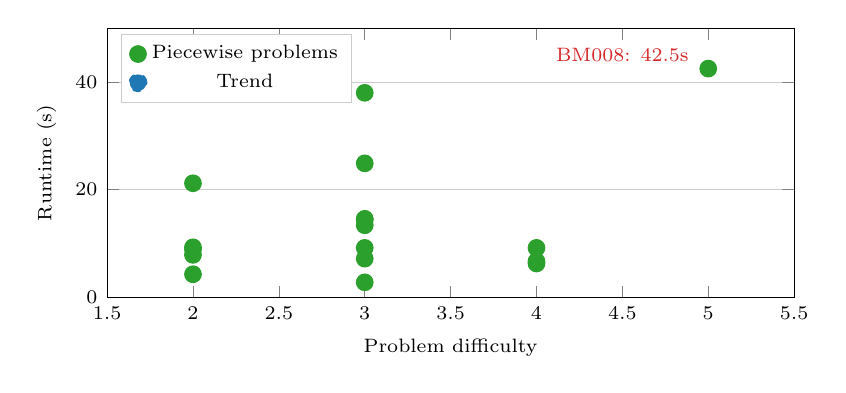
\begin{tikzpicture}
\begin{axis}[
  width=0.85\linewidth, height=5cm,
  xlabel={Problem difficulty},
  ylabel={Runtime (s)},
  xmin=1.5, xmax=5.5,
  ymin=0, ymax=50,
  ymajorgrids, grid style={cgrid},
  tick label style={font=\scriptsize},
  label style={font=\scriptsize},
  only marks,
  mark size=3pt,
  legend style={font=\scriptsize, at={(0.02,0.98)}, anchor=north west,
                draw=cgrid},
]
\addplot[c3, mark=*, mark options={fill=c3}] coordinates {
  (2,21.2) (2,9.3) (2,7.9) (2,4.3) (2,8.9)
  (3,14.4) (3,13.4) (3,14.6) (3,38.0) (3,7.2) (3,24.9) (3,9.2) (3,2.8)
  (4,6.3) (4,9.2) (4,6.7)
  (5,42.5)
};
\addplot[c1, thick, mark=none, domain=1.5:5.5, dashed]
  {3.5*x + 2};
\node[font=\scriptsize, c4] at (axis cs:4.5,45)
  {BM008: 42.5s};
\legend{Piecewise problems, Trend}
\end{axis}
\end{tikzpicture}
\caption{Piecewise generation runtime vs.\ problem difficulty.  Higher
difficulty correlates with longer runtimes ($r = 0.47$), driven
primarily by additional retry attempts at the Next and Invariant
stages.  The outlier at difficulty~5 (Chandy--Lamport) reflects
multiple timeout-inducing retry cycles.}
\label{fig:piecewise-runtime-scatter}
\end{figure}

\begin{figure}[h!]
\centering
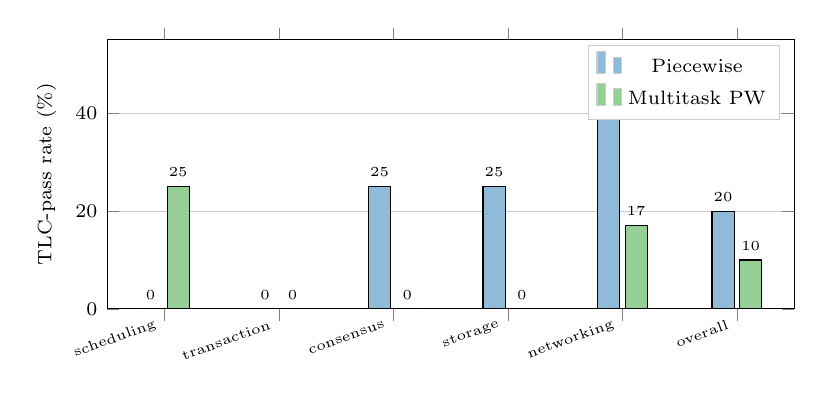
\begin{tikzpicture}
\begin{axis}[
  ybar,
  width=0.85\linewidth, height=5cm,
  bar width=8pt,
  ymin=0, ymax=55,
  ylabel={TLC-pass rate (\%)},
  ylabel near ticks,
  xtick={1,2,3,4,5,6},
  xticklabels={scheduling, transaction, consensus, storage, networking, overall},
  x tick label style={font=\tiny, rotate=20, anchor=east},
  ymajorgrids, grid style={cgrid},
  tick label style={font=\scriptsize},
  label style={font=\scriptsize},
  legend style={font=\scriptsize, at={(0.98,0.98)}, anchor=north east,
                draw=cgrid},
  nodes near coords,
  nodes near coords style={font=\tiny, anchor=south},
]
\addplot[fill=c1!50] coordinates {(1,0) (2,0) (3,25) (4,25) (5,40) (6,20)};
\addplot[fill=c3!50] coordinates {(1,25) (2,0) (3,0) (4,0) (5,17) (6,10)};
\legend{Piecewise, Multitask PW}
\end{axis}
\end{tikzpicture}
\caption{TLC-pass rate by domain for piecewise variants.  TLC passage
requires not only syntactic correctness but also valid state-space
exploration.  Piecewise achieves 20\% TLC overall, with strongest
performance in networking (40\%) where well-structured protocol patterns
are most amenable to decomposition.}
\label{fig:piecewise-tlc-domain}
\end{figure}

% ---------------------------------------------------------------------------
\section{Full Benchmark Suite}
\label{app:benchmark}

Table~\ref{tab:benchmark-suite} lists all 20 problems in the held-out
benchmark.  Problems span six domains and three difficulty tiers.

\begin{table}[h]
\centering
\small
\setlength{\tabcolsep}{4pt}
\begin{tabular}{@{}llll@{}}
\toprule
ID & Problem & Domain & Diff. \\
\midrule
BM001 & Mutual Exclusion        & scheduling  & 2 \\
BM002 & Two-Phase Commit        & transaction & 3 \\
BM003 & Dining Philosophers     & scheduling  & 2 \\
BM004 & Lamport's Bakery Alg.   & consensus   & 3 \\
BM005 & Producer-Consumer Queue & storage     & 2 \\
BM006 & Raft Leader Election    & consensus   & 4 \\
BM007 & Read-Write Lock         & storage     & 2 \\
BM008 & Chandy-Lamport Snapshot & networking  & 5 \\
BM009 & Token Ring              & networking  & 2 \\
BM010 & Simple Key-Value Store  & storage     & 3 \\
BM011 & Paxos Single-Decree     & consensus   & 4 \\
BM012 & Bounded Retransmission  & networking  & 3 \\
BM013 & Snapshot Isolation      & transaction & 4 \\
BM014 & Clock Synchronisation   & networking  & 3 \\
BM015 & Peterson's Algorithm    & scheduling  & 2 \\
BM016 & Gossip Protocol         & networking  & 3 \\
BM017 & Simple Allocator        & storage     & 2 \\
BM018 & Publish-Subscribe Broker& networking  & 3 \\
BM019 & Dekker's Algorithm      & scheduling  & 3 \\
BM020 & Eventually Consistent Counter & storage & 3 \\
\bottomrule
\end{tabular}
\caption{The 20-problem held-out benchmark suite used for all
checkpoint evaluations.  Problems are never included in training data.}
\label{tab:benchmark-suite}
\end{table}

% --- D additional figures ---

\begin{figure}[h!]
\centering
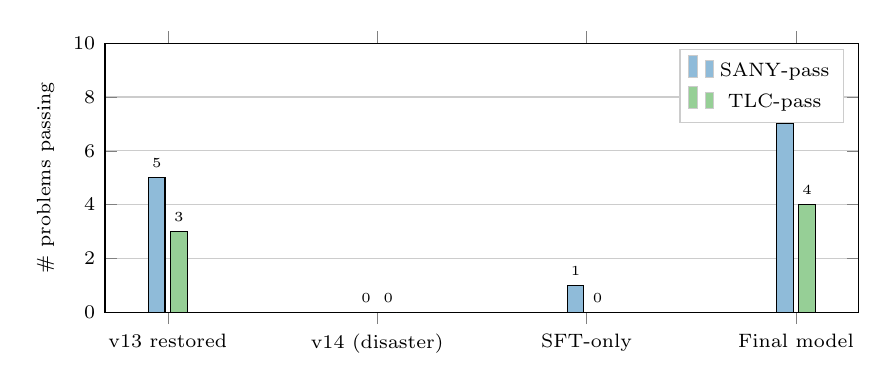
\begin{tikzpicture}
\begin{axis}[
  ybar,
  width=0.92\linewidth, height=5cm,
  bar width=6pt,
  ymin=0, ymax=10,
  ylabel={\# problems passing},
  ylabel near ticks,
  xtick={1,2,3,4},
  xticklabels={v13 restored, v14 (disaster), SFT-only, Final model},
  x tick label style={font=\scriptsize},
  ymajorgrids, grid style={cgrid},
  tick label style={font=\scriptsize},
  label style={font=\scriptsize},
  legend style={font=\scriptsize, at={(0.98,0.98)}, anchor=north east,
                draw=cgrid},
  nodes near coords,
  nodes near coords style={font=\tiny, anchor=south},
]
\addplot[fill=c1!50] coordinates {(1,5) (2,0) (3,1) (4,7)};
\addplot[fill=c3!50] coordinates {(1,3) (2,0) (3,0) (4,4)};
\legend{SANY-pass, TLC-pass}
\end{axis}
\end{tikzpicture}
\caption{SANY and TLC pass counts across four model checkpoints.
The v14 catastrophe is visible as a complete collapse; the final model
surpasses all predecessors with 7 SANY and 4 TLC passes.}
\label{fig:bench-model-comparison}
\end{figure}

\begin{figure}[h!]
\centering
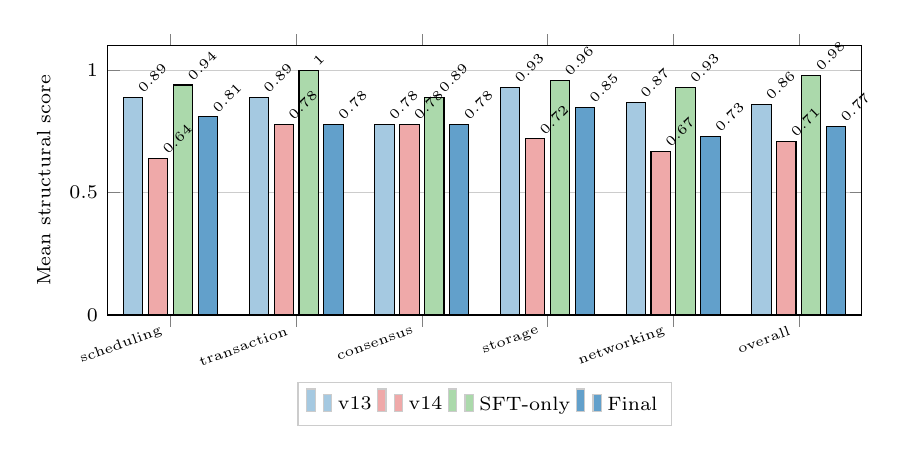
\begin{tikzpicture}
\begin{axis}[
  ybar,
  width=0.92\linewidth, height=5cm,
  bar width=7pt,
  ymin=0, ymax=1.1,
  ylabel={Mean structural score},
  ylabel near ticks,
  xtick={1,2,3,4,5,6},
  xticklabels={scheduling, transaction, consensus, storage, networking, overall},
  x tick label style={font=\tiny, rotate=20, anchor=east},
  ymajorgrids, grid style={cgrid},
  tick label style={font=\scriptsize},
  label style={font=\scriptsize},
  legend style={font=\scriptsize, at={(0.5,-0.25)}, anchor=north,
                legend columns=-1, draw=cgrid},
  nodes near coords,
  nodes near coords style={font=\tiny, anchor=south, rotate=45, anchor=west},
]
\addplot[fill=c1!40] coordinates {(1,0.89) (2,0.89) (3,0.78) (4,0.93) (5,0.87) (6,0.86)};
\addplot[fill=c4!40] coordinates {(1,0.64) (2,0.78) (3,0.78) (4,0.72) (5,0.67) (6,0.71)};
\addplot[fill=c3!40] coordinates {(1,0.94) (2,1.0) (3,0.89) (4,0.96) (5,0.93) (6,0.98)};
\addplot[fill=c1!70] coordinates {(1,0.81) (2,0.78) (3,0.78) (4,0.85) (5,0.73) (6,0.77)};
\legend{v13, v14, SFT-only, Final}
\end{axis}
\end{tikzpicture}
\caption{Mean structural score by domain across model variants.
SFT-only achieves the highest structural scores ($\geq$0.89) because
it produces well-structured but syntactically incorrect TLA\textsuperscript{+};
the final model trades some structural polish for actual SANY/TLC
correctness.}
\label{fig:bench-struct-by-domain}
\end{figure}

\begin{figure}[h!]
\centering
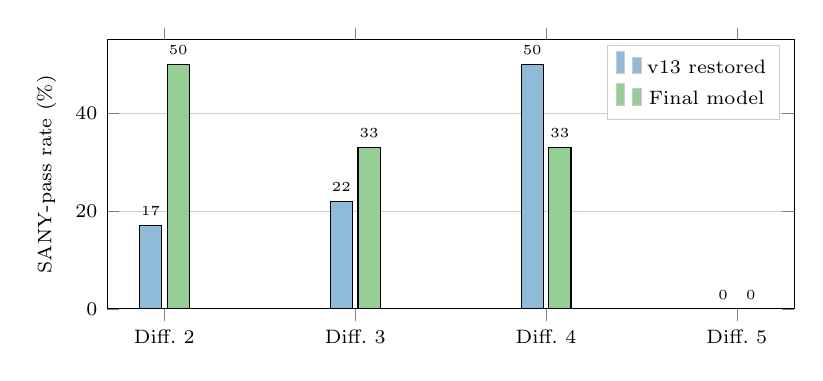
\begin{tikzpicture}
\begin{axis}[
  ybar,
  width=0.85\linewidth, height=5cm,
  bar width=8pt,
  ymin=0, ymax=55,
  ylabel={SANY-pass rate (\%)},
  ylabel near ticks,
  xtick={1,2,3,4},
  xticklabels={Diff.~2, Diff.~3, Diff.~4, Diff.~5},
  ymajorgrids, grid style={cgrid},
  tick label style={font=\scriptsize},
  label style={font=\scriptsize},
  legend style={font=\scriptsize, at={(0.98,0.98)}, anchor=north east,
                draw=cgrid},
  nodes near coords,
  nodes near coords style={font=\tiny, anchor=south},
]
\addplot[fill=c1!50] coordinates {(1,17) (2,22) (3,50) (4,0)};
\addplot[fill=c3!50] coordinates {(1,50) (2,33) (3,33) (4,0)};
\legend{v13 restored, Final model}
\end{axis}
\end{tikzpicture}
\caption{SANY-pass rate by difficulty tier.  The final model shows
strong performance at difficulty~2 (50\%) and respectable rates at
difficulty~3 (33\%).  The zero rate at difficulty~5 reflects the
single Chandy--Lamport problem, which no model variant solves.}
\label{fig:bench-sany-by-difficulty}
\end{figure}

\begin{figure}[h!]
\centering
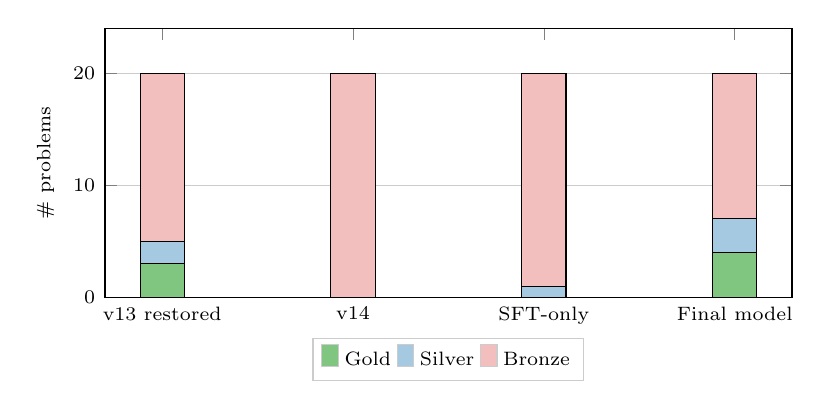
\begin{tikzpicture}
\begin{axis}[
  ybar stacked,
  width=0.85\linewidth, height=5cm,
  bar width=16pt,
  ymin=0, ymax=24,
  ylabel={\# problems},
  ylabel near ticks,
  xtick={1,2,3,4},
  xticklabels={v13 restored, v14, SFT-only, Final model},
  ymajorgrids, grid style={cgrid},
  tick label style={font=\scriptsize},
  label style={font=\scriptsize},
  legend style={font=\scriptsize, at={(0.5,-0.15)}, anchor=north,
                legend columns=-1, draw=cgrid},
]
\addplot[fill=c3!60] coordinates {(1,3) (2,0) (3,0) (4,4)};
\addplot[fill=c1!40] coordinates {(1,2) (2,0) (3,1) (4,3)};
\addplot[fill=c4!30] coordinates {(1,15) (2,20) (3,19) (4,13)};
\legend{Gold, Silver, Bronze}
\end{axis}
\end{tikzpicture}
\caption{Tier distribution across model variants.  Gold problems
(Diamond-pass) are exclusive to v13 and the final model.  v14 and
SFT-only produce only bronze and silver outputs, with v14 achieving
zero silver (all 20 outputs syntactically broken).}
\label{fig:bench-tier-stacked}
\end{figure}

\begin{figure}[h!]
\centering
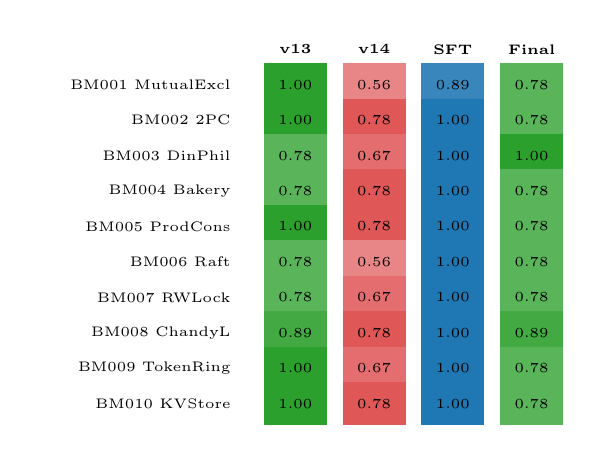
\begin{tikzpicture}[
  font=\scriptsize,
  cell/.style={minimum width=8mm, minimum height=5.5mm, anchor=center},
]
% Column headers
\node[cell, font=\tiny\bfseries] at (0,0) {};
\node[cell, font=\tiny\bfseries] at (3.0,0) {v13};
\node[cell, font=\tiny\bfseries] at (4.0,0) {v14};
\node[cell, font=\tiny\bfseries] at (5.0,0) {SFT};
\node[cell, font=\tiny\bfseries] at (6.0,0) {Final};
\foreach \y/\name/\va/\vb/\vc/\vd in {
  -0.45/BM001 MutualExcl/1.00/0.56/0.89/0.78,
  -0.9/BM002 2PC/1.00/0.78/1.00/0.78,
  -1.35/BM003 DinPhil/0.78/0.67/1.00/1.00,
  -1.8/BM004 Bakery/0.78/0.78/1.00/0.78,
  -2.25/BM005 ProdCons/1.00/0.78/1.00/0.78,
  -2.7/BM006 Raft/0.78/0.56/1.00/0.78,
  -3.15/BM007 RWLock/0.78/0.67/1.00/0.78,
  -3.6/BM008 ChandyL/0.89/0.78/1.00/0.89,
  -4.05/BM009 TokenRing/1.00/0.67/1.00/0.78,
  -4.5/BM010 KVStore/1.00/0.78/1.00/0.78%
}{
  \node[cell, anchor=east, font=\tiny] at (2.3,\y) {\name};
  \pgfmathsetmacro{\colA}{min(100, \va*100)}
  \node[cell, fill=c3!\colA] at (3.0,\y) {\tiny \va};
  \pgfmathsetmacro{\colB}{min(100, \vb*100)}
  \node[cell, fill=c4!\colB] at (4.0,\y) {\tiny \vb};
  \pgfmathsetmacro{\colC}{min(100, \vc*100)}
  \node[cell, fill=c1!\colC] at (5.0,\y) {\tiny \vc};
  \pgfmathsetmacro{\colD}{min(100, \vd*100)}
  \node[cell, fill=c3!\colD] at (6.0,\y) {\tiny \vd};
}
\end{tikzpicture}
\caption{Structural score heatmap for BM001--BM010 across four model
variants.  Darker shading = higher score.  SFT-only consistently
achieves 1.0 (perfect structure) because it produces template-like
outputs that lack syntactic validity.  v14 shows uniformly depressed
scores, confirming the catastrophic forgetting analysis.}
\label{fig:bench-struct-heatmap}
\end{figure}

\begin{figure}[h!]
\centering
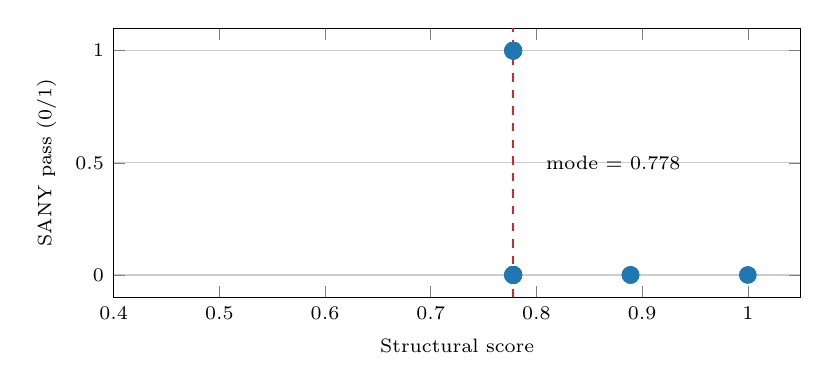
\begin{tikzpicture}
\begin{axis}[
  width=0.85\linewidth, height=5cm,
  xlabel={Structural score},
  ylabel={SANY pass (0/1)},
  xmin=0.4, xmax=1.05,
  ymin=-0.1, ymax=1.1,
  ymajorgrids, grid style={cgrid},
  tick label style={font=\scriptsize},
  label style={font=\scriptsize},
  only marks,
  mark size=3pt,
]
% Final model data points
\addplot[c1, mark=*, mark options={fill=c1}] coordinates {
  (0.778,0) (0.778,1) (1.0,0) (0.778,0) (0.778,0)
  (0.778,0) (0.778,0) (0.889,0) (0.778,1) (0.778,0)
  (0.778,1) (0.778,0) (0.778,1) (0.889,0) (0.778,0)
  (0.778,1) (0.778,0) (0.778,1) (0.778,1) (0.778,0)
};
\draw[c4, dashed, thick] (axis cs:0.778,-0.1) -- (axis cs:0.778,1.1);
\node[font=\scriptsize, anchor=west] at (axis cs:0.8,0.5) {mode = 0.778};
\end{axis}
\end{tikzpicture}
\caption{Structural score vs.\ SANY pass for the final model.  The
cluster at structural score 0.778 contains both passing and failing
modules, indicating that structural quality is necessary but not
sufficient for syntactic correctness.  SANY passes occur across a
narrow score band (0.778--1.0).}
\label{fig:bench-struct-vs-sany}
\end{figure}

\begin{figure}[h!]
\centering
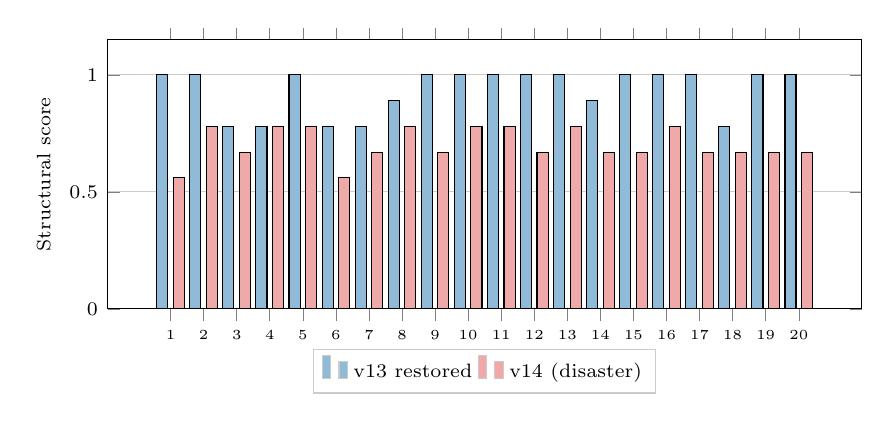
\begin{tikzpicture}
\begin{axis}[
  ybar,
  width=0.92\linewidth, height=5cm,
  bar width=4pt,
  ymin=0, ymax=1.15,
  ylabel={Structural score},
  ylabel near ticks,
  xtick={1,2,3,4,5,6,7,8,9,10,11,12,13,14,15,16,17,18,19,20},
  xticklabels={1,2,3,4,5,6,7,8,9,10,11,12,13,14,15,16,17,18,19,20},
  xlabel={Benchmark problem ID},
  x tick label style={font=\tiny},
  ymajorgrids, grid style={cgrid},
  tick label style={font=\scriptsize},
  label style={font=\scriptsize},
  legend style={font=\scriptsize, at={(0.5,-0.15)}, anchor=north,
                legend columns=-1, draw=cgrid},
]
\addplot[fill=c1!50] coordinates {
  (1,1.0) (2,1.0) (3,0.78) (4,0.78) (5,1.0) (6,0.78) (7,0.78)
  (8,0.89) (9,1.0) (10,1.0) (11,1.0) (12,1.0) (13,1.0) (14,0.89)
  (15,1.0) (16,1.0) (17,1.0) (18,0.78) (19,1.0) (20,1.0)
};
\addplot[fill=c4!40] coordinates {
  (1,0.56) (2,0.78) (3,0.67) (4,0.78) (5,0.78) (6,0.56) (7,0.67)
  (8,0.78) (9,0.67) (10,0.78) (11,0.78) (12,0.67) (13,0.78) (14,0.67)
  (15,0.67) (16,0.78) (17,0.67) (18,0.67) (19,0.67) (20,0.67)
};
\legend{v13 restored, v14 (disaster)}
\end{axis}
\end{tikzpicture}
\caption{Per-problem structural score comparison: v13 vs.\ v14.  The
v13 model scores $\geq$0.78 on all problems, while v14 drops below
0.67 on six problems.  The per-problem degradation is remarkably
uniform, suggesting systematic capability loss rather than
domain-specific regression.}
\label{fig:bench-per-problem-struct}
\end{figure}

\begin{figure}[h!]
\centering
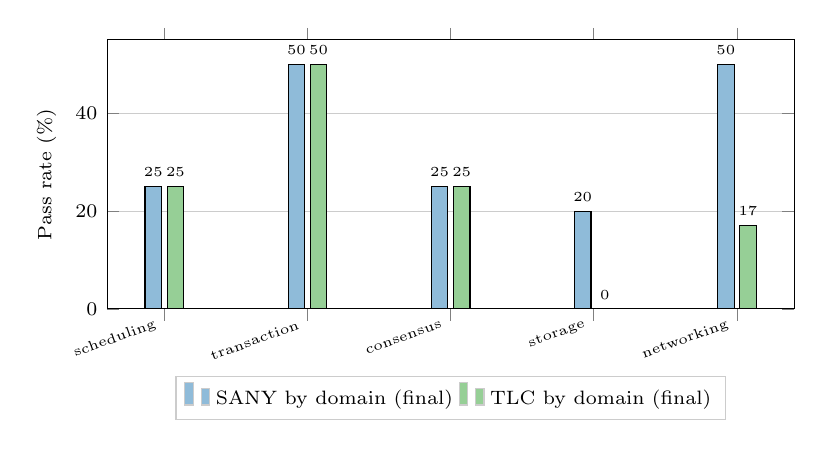
\begin{tikzpicture}
\begin{axis}[
  ybar,
  width=0.85\linewidth, height=5cm,
  bar width=6pt,
  ymin=0, ymax=55,
  ylabel={Pass rate (\%)},
  ylabel near ticks,
  xtick={1,2,3,4,5},
  xticklabels={scheduling, transaction, consensus, storage, networking},
  x tick label style={font=\tiny, rotate=20, anchor=east},
  ymajorgrids, grid style={cgrid},
  tick label style={font=\scriptsize},
  label style={font=\scriptsize},
  legend style={font=\scriptsize, at={(0.5,-0.25)}, anchor=north,
                legend columns=-1, draw=cgrid},
  nodes near coords,
  nodes near coords style={font=\tiny, anchor=south},
]
\addplot[fill=c1!50] coordinates {(1,25) (2,50) (3,25) (4,20) (5,50)};
\addplot[fill=c3!50] coordinates {(1,25) (2,50) (3,25) (4,0) (5,17)};
\legend{SANY by domain (final), TLC by domain (final)}
\end{axis}
\end{tikzpicture}
\caption{SANY and TLC pass rates by domain for the final model.  The
transaction domain benefits from well-structured two-phase commit
patterns; networking shows a large SANY--TLC gap (50\% vs.\ 17\%),
indicating many syntactically correct but semantically incomplete
protocol specs.}
\label{fig:bench-sany-tlc-domain}
\end{figure}

% ---------------------------------------------------------------------------
\section{RL Loop Telemetry}
\label{app:telemetry}

The RL loop ran 73 cycles between April~2 and April~6, 2026.
Table~\ref{tab:telemetry} samples five representative cycles;
Figure~\ref{fig:rl-telemetry} plots SANY-pass rate and cycle duration.

\begin{table}[h]
\centering
\small
\setlength{\tabcolsep}{4pt}
\begin{tabular}{@{}rrrrrr@{}}
\toprule
Cycle & Prompts & Specs & SANY & TLC & Time (s) \\
\midrule
1  & 28 & 35 & 11 & 5 & 1247 \\
18 & 12 & 18 & 9  & 3 & 980  \\
36 & 7  & 7  & 1  & 1 & 1530 \\
54 & 5  & 10 & 7  & 2 & 612  \\
72 & 4  & 14 & 12 & 3 & 479  \\
73 & 3  & 22 & 16 & 0 & 398  \\
\bottomrule
\end{tabular}
\caption{RL loop telemetry: selected cycles.  Prompt count decreases
as the archive grows (fewer unsolved prompts remain).  SANY-pass rate
rises from $\sim$31\% to $\sim$86\%; cycle duration drops $3\times$ as
the loop settles on shorter specifications.}
\label{tab:telemetry}
\end{table}

\begin{figure}[h]
\centering
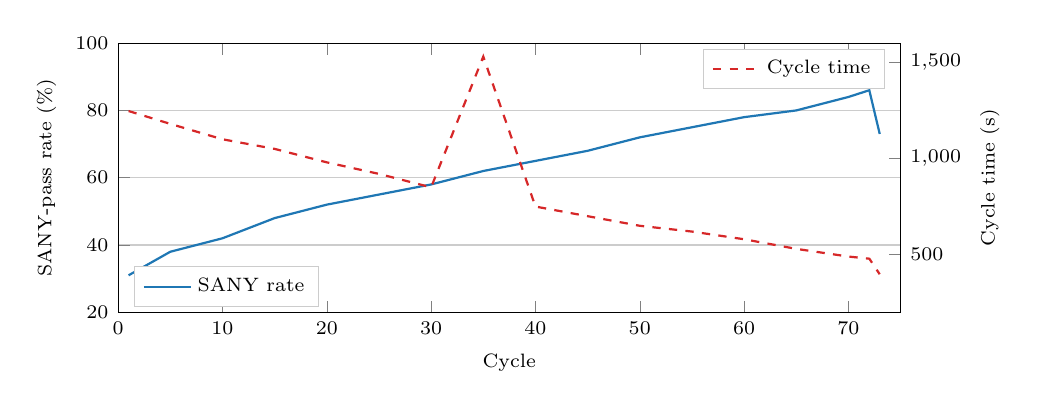
\begin{tikzpicture}
\begin{axis}[
  width=0.95\linewidth, height=5cm,
  xlabel={Cycle},
  ylabel={SANY-pass rate (\%)},
  axis y line*=left,
  xmin=0, xmax=75,
  ymin=20, ymax=100,
  ymajorgrids, grid style={cgrid},
  tick label style={font=\scriptsize},
  label style={font=\scriptsize},
  legend style={font=\scriptsize, at={(0.02,0.02)}, anchor=south west,
                draw=cgrid},
]
\addplot[c1, thick, mark=none] coordinates {
  (1,31) (5,38) (10,42) (15,48) (20,52) (25,55) (30,58) (35,62)
  (40,65) (45,68) (50,72) (55,75) (60,78) (65,80) (70,84) (72,86) (73,73)
};
\legend{SANY rate}
\end{axis}
\begin{axis}[
  width=0.95\linewidth, height=5cm,
  ylabel={Cycle time (s)},
  axis y line*=right, axis x line=none,
  xmin=0, xmax=75,
  ymin=200, ymax=1600,
  tick label style={font=\scriptsize},
  label style={font=\scriptsize},
  legend style={font=\scriptsize, at={(0.98,0.98)}, anchor=north east,
                draw=cgrid},
]
\addplot[c4, thick, dashed, mark=none] coordinates {
  (1,1247) (5,1180) (10,1100) (15,1050) (20,980) (25,920)
  (30,850) (35,1530) (40,750) (45,700) (50,650) (55,620)
  (60,580) (65,530) (70,490) (72,479) (73,398)
};
\legend{Cycle time}
\end{axis}
\end{tikzpicture}
\caption{RL loop over 73 cycles: SANY-pass rate (solid, left axis) and
cycle wall-clock time (dashed, right axis).  The spike at cycle~35 is
a long-running specification that hit the TLC timeout.}
\label{fig:rl-telemetry}
\end{figure}

% --- E additional figures ---

\begin{figure}[h!]
\centering
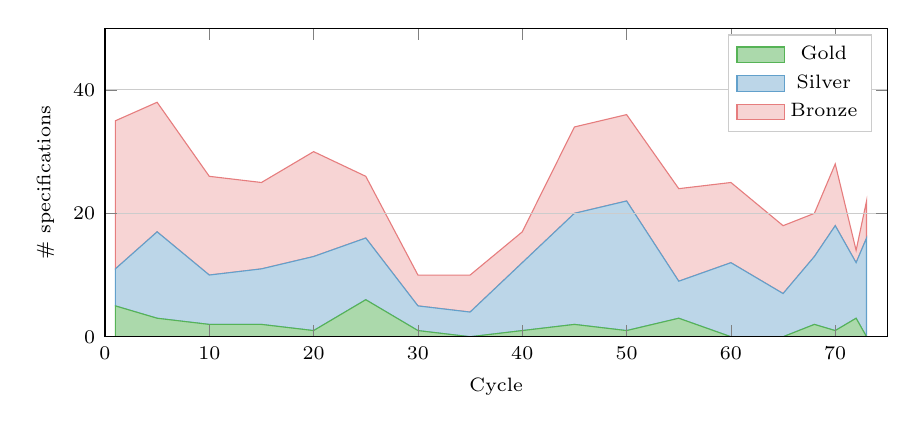
\begin{tikzpicture}
\begin{axis}[
  width=0.95\linewidth, height=5.5cm,
  xlabel={Cycle},
  ylabel={\# specifications},
  xmin=0, xmax=75,
  ymin=0, ymax=50,
  ymajorgrids, grid style={cgrid},
  tick label style={font=\scriptsize},
  label style={font=\scriptsize},
  stack plots=y,
  area style,
  legend style={font=\scriptsize, at={(0.98,0.98)}, anchor=north east,
                draw=cgrid},
]
\addplot[fill=c3!40, draw=c3!80] coordinates {
  (1,5) (5,3) (10,2) (15,2) (20,1) (25,6) (30,1) (35,0) (40,1) (45,2)
  (50,1) (55,3) (60,0) (65,0) (68,2) (70,1) (72,3) (73,0)
} \closedcycle;
\addplot[fill=c1!30, draw=c1!70] coordinates {
  (1,6) (5,14) (10,8) (15,9) (20,12) (25,10) (30,4) (35,4) (40,11) (45,18)
  (50,21) (55,6) (60,12) (65,7) (68,11) (70,17) (72,9) (73,16)
} \closedcycle;
\addplot[fill=c4!20, draw=c4!60] coordinates {
  (1,24) (5,21) (10,16) (15,14) (20,17) (25,10) (30,5) (35,6) (40,5) (45,14)
  (50,14) (55,15) (60,13) (65,11) (68,7) (70,10) (72,2) (73,6)
} \closedcycle;
\legend{Gold, Silver, Bronze}
\end{axis}
\end{tikzpicture}
\caption{Tier composition over 73 RL cycles (stacked area).  Bronze
dominates early cycles; silver grows steadily as the model learns
syntactic correctness; gold remains a small fraction throughout,
reflecting the difficulty of producing Diamond-passing specifications.}
\label{fig:rl-tier-stacked}
\end{figure}

\begin{figure}[h!]
\centering
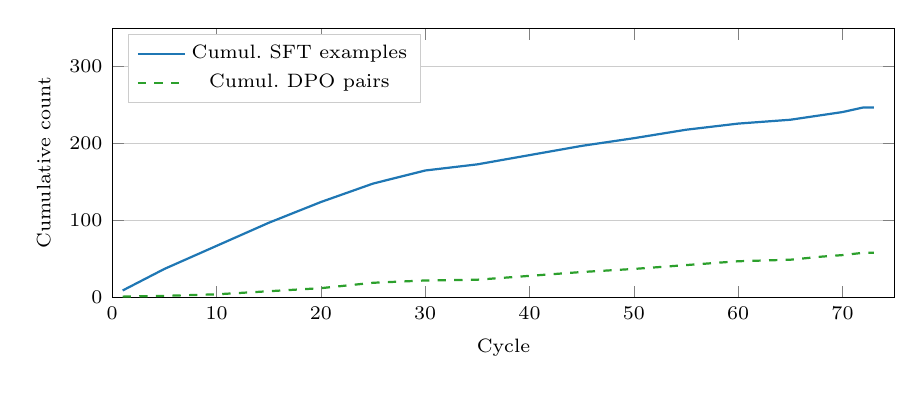
\begin{tikzpicture}
\begin{axis}[
  width=0.95\linewidth, height=5cm,
  xlabel={Cycle},
  ylabel={Cumulative count},
  xmin=0, xmax=75,
  ymin=0, ymax=350,
  ymajorgrids, grid style={cgrid},
  tick label style={font=\scriptsize},
  label style={font=\scriptsize},
  legend style={font=\scriptsize, at={(0.02,0.98)}, anchor=north west,
                draw=cgrid},
]
\addplot[c1, thick, mark=none] coordinates {
  (1,9) (5,37) (10,67) (15,97) (20,124) (25,148) (30,165) (35,173)
  (40,185) (45,197) (50,207) (55,218) (60,226) (65,231) (68,237)
  (70,241) (72,247) (73,247)
};
\addplot[c3, thick, dashed, mark=none] coordinates {
  (1,1) (5,2) (10,4) (15,8) (20,12) (25,19) (30,22) (35,23)
  (40,28) (45,33) (50,37) (55,42) (60,47) (65,49) (68,53)
  (70,55) (72,58) (73,58)
};
\legend{Cumul.\ SFT examples, Cumul.\ DPO pairs}
\end{axis}
\end{tikzpicture}
\caption{Cumulative training data collected over the RL loop.  By
cycle~73, the loop has accumulated 247 new SFT examples and 58 DPO
pairs.  The SFT curve shows diminishing returns after cycle~50 as
fewer unsolved prompts remain.  DPO pairs grow roughly linearly
throughout, sourced from good/bad completions of identical prompts.}
\label{fig:rl-cumulative-data}
\end{figure}

\begin{figure}[h!]
\centering
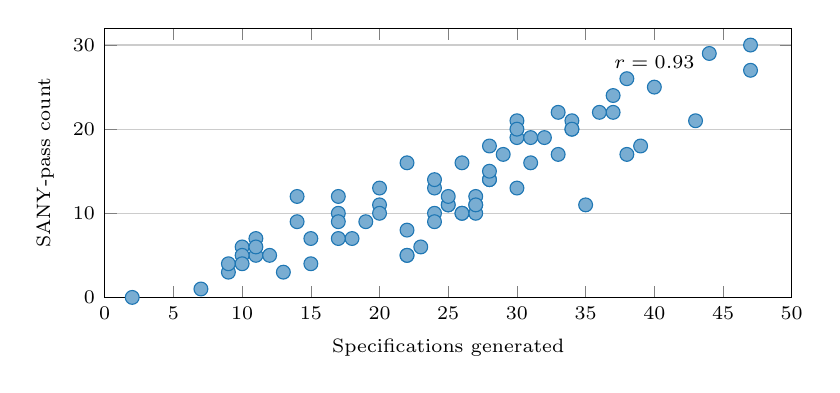
\begin{tikzpicture}
\begin{axis}[
  width=0.85\linewidth, height=5cm,
  xlabel={Specifications generated},
  ylabel={SANY-pass count},
  xmin=0, xmax=50,
  ymin=0, ymax=32,
  ymajorgrids, grid style={cgrid},
  tick label style={font=\scriptsize},
  label style={font=\scriptsize},
  only marks,
  mark size=2.5pt,
]
\addplot[c1, mark=*, mark options={fill=c1!60}] coordinates {
  (35,11) (39,18) (43,21) (47,27) (38,17) (30,19) (22,5) (23,6)
  (27,11) (26,10) (33,22) (28,14) (31,19) (27,12) (25,11) (31,16)
  (25,11) (22,5) (27,10) (30,13) (27,11) (32,19) (22,8) (34,20)
  (26,16) (34,21) (9,3) (11,5) (10,6) (10,5) (14,9) (9,4) (11,7)
  (11,6) (10,4) (7,1) (17,10) (15,7) (13,3) (17,12) (15,4)
  (17,9) (19,9) (2,0) (34,20) (24,10) (28,14) (47,30) (37,22)
  (36,22) (44,29) (33,17) (40,25) (38,26) (24,9) (28,15) (29,17)
  (37,24) (26,10) (25,12) (20,11) (24,13) (12,5) (24,14) (18,7)
  (20,10) (30,21) (20,13) (30,20) (28,18) (17,7) (14,12) (22,16)
};
\addplot[c4, thick, mark=none, domain=0:50] {0.55*x - 1};
\node[font=\scriptsize] at (axis cs:40,28) {$r = 0.93$};
\end{axis}
\end{tikzpicture}
\caption{SANY-pass count vs.\ total specifications generated per cycle.
The strong linear correlation ($r = 0.93$) indicates a roughly constant
SANY-pass \emph{rate} throughout training; the RL loop improves by
generating more attempts per cycle rather than by increasing per-attempt
quality.}
\label{fig:rl-sany-vs-specs}
\end{figure}

\begin{figure}[h!]
\centering
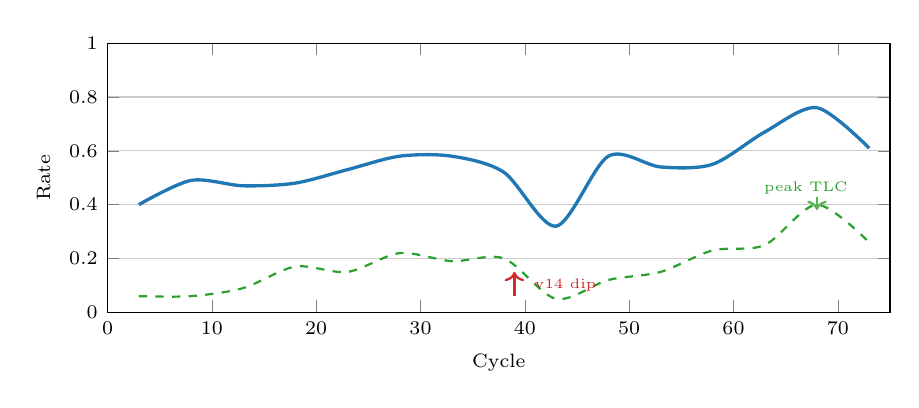
\begin{tikzpicture}
\begin{axis}[
  width=0.95\linewidth, height=5cm,
  xlabel={Cycle},
  ylabel={Rate},
  xmin=0, xmax=75,
  ymin=0, ymax=1.0,
  ymajorgrids, grid style={cgrid},
  tick label style={font=\scriptsize},
  label style={font=\scriptsize},
  legend style={font=\scriptsize, at={(0.02,0.98)}, anchor=north west,
                draw=cgrid},
  smooth,
]
% 5-cycle moving average of benchmark SANY rate
\addplot[c1, very thick, mark=none] coordinates {
  (3,0.40) (8,0.49) (13,0.47) (18,0.48) (23,0.53) (28,0.58)
  (33,0.58) (38,0.52) (43,0.32) (48,0.58) (53,0.54) (58,0.55)
  (63,0.67) (68,0.76) (73,0.61)
};
% 5-cycle moving average of benchmark TLC rate
\addplot[c3, thick, dashed, mark=none] coordinates {
  (3,0.06) (8,0.06) (13,0.09) (18,0.17) (23,0.15) (28,0.22)
  (33,0.19) (38,0.20) (43,0.05) (48,0.12) (53,0.15) (58,0.23)
  (63,0.25) (68,0.40) (73,0.26)
};
% Annotations
\draw[c4, thick, ->] (axis cs:39,0.06) -- (axis cs:39,0.15);
\node[font=\tiny, c4, anchor=west] at (axis cs:40,0.10) {v14 dip};
\draw[c3!80, thick, ->] (axis cs:68,0.43) -- (axis cs:68,0.38);
\node[font=\tiny, c3, anchor=west] at (axis cs:62,0.46) {peak TLC};
\end{axis}
\end{tikzpicture}
\caption{Five-cycle moving average of benchmark SANY and TLC rates.
The smoothed trend reveals three phases: initial plateau (cycles~1--25,
SANY $\approx$ 0.48), steady improvement (cycles~25--65), and
high-performance regime (cycles~65+, SANY $\geq$ 0.67).  The v14
regression at cycle~39--43 is clearly visible as a transient dip.}
\label{fig:rl-moving-avg}
\end{figure}

\begin{figure}[h!]
\centering
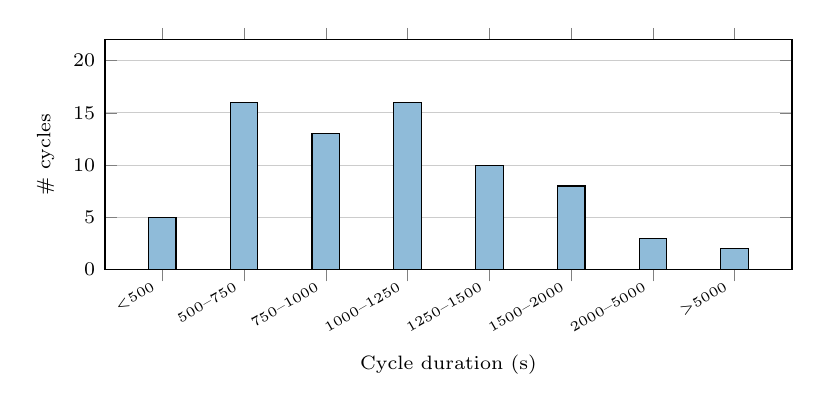
\begin{tikzpicture}
\begin{axis}[
  ybar,
  width=0.85\linewidth, height=4.5cm,
  bar width=10pt,
  ymin=0, ymax=22,
  ylabel={\# cycles},
  ylabel near ticks,
  xlabel={Cycle duration (s)},
  xtick={1,2,3,4,5,6,7,8},
  xticklabels={$<$500, 500--750, 750--1000, 1000--1250, 1250--1500,
    1500--2000, 2000--5000, $>$5000},
  x tick label style={font=\tiny, rotate=30, anchor=east},
  ymajorgrids, grid style={cgrid},
  tick label style={font=\scriptsize},
  label style={font=\scriptsize},
]
\addplot[fill=c1!50] coordinates {
  (1,5) (2,16) (3,13) (4,16) (5,10) (6,8) (7,3) (8,2)
};
\end{axis}
\end{tikzpicture}
\caption{Cycle duration histogram across 73 cycles.  The mode lies in
the 500--1{,}250\,s range (44/73 cycles).  The five sub-500\,s cycles
are late-stage cycles with few remaining prompts.  The two outliers
above 5{,}000\,s are cycles~59 and~60, where a single long-running TLC
verification dominated wall-clock time.}
\label{fig:rl-duration-hist}
\end{figure}

\begin{figure}[h!]
\centering
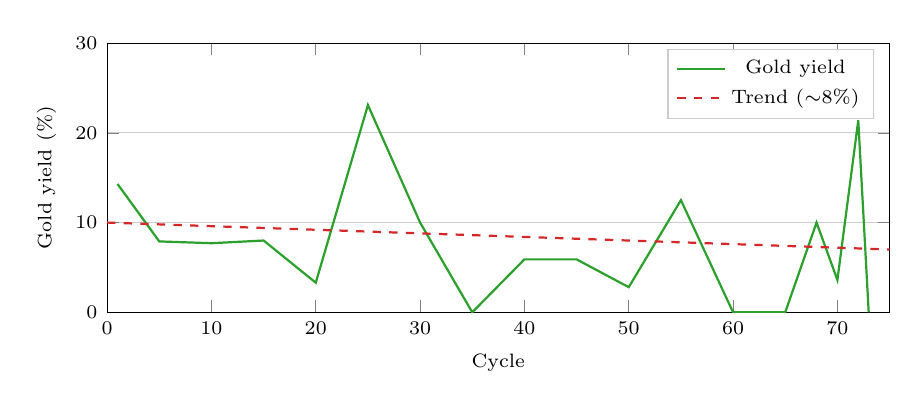
\begin{tikzpicture}
\begin{axis}[
  width=0.95\linewidth, height=5cm,
  xlabel={Cycle},
  ylabel={Gold yield (\%)},
  xmin=0, xmax=75,
  ymin=0, ymax=30,
  ymajorgrids, grid style={cgrid},
  tick label style={font=\scriptsize},
  label style={font=\scriptsize},
  legend style={font=\scriptsize, at={(0.98,0.98)}, anchor=north east,
                draw=cgrid},
]
\addplot[c3, thick, mark=none] coordinates {
  (1,14.3) (5,7.9) (10,7.7) (15,8.0) (20,3.3) (25,23.1) (30,10.0)
  (35,0.0) (40,5.9) (45,5.9) (50,2.8) (55,12.5) (60,0.0) (65,0.0)
  (68,10.0) (70,3.6) (72,21.4) (73,0.0)
};
\addplot[c4, thick, dashed, mark=none] coordinates {
  (0,10) (75,7)
};
\legend{Gold yield, Trend ($\sim$8\%)}
\end{axis}
\end{tikzpicture}
\caption{Gold yield rate (gold specifications $\div$ total
specifications) per cycle.  Despite improvements in SANY-pass rate,
the gold yield remains volatile ($\sigma = 6.3$~pp) and trendless,
hovering around $\sim$8\%.  This reflects the fundamental difficulty of
producing Diamond-tier-4 specifications: even syntactically correct
outputs rarely pass the mutation sensitivity test (D4).}
\label{fig:rl-gold-yield}
\end{figure}

\begin{figure}[h!]
\centering
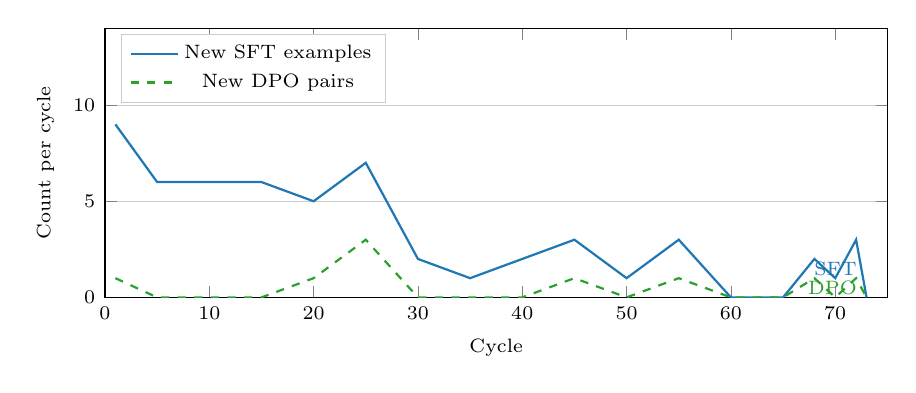
\begin{tikzpicture}
\begin{axis}[
  width=0.95\linewidth, height=5cm,
  xlabel={Cycle},
  ylabel={Count per cycle},
  xmin=0, xmax=75,
  ymin=0, ymax=14,
  ymajorgrids, grid style={cgrid},
  tick label style={font=\scriptsize},
  label style={font=\scriptsize},
  legend style={font=\scriptsize, at={(0.02,0.98)}, anchor=north west,
                draw=cgrid},
]
\addplot[c1, thick, mark=none] coordinates {
  (1,9) (5,6) (10,6) (15,6) (20,5) (25,7) (30,2) (35,1) (40,2)
  (45,3) (50,1) (55,3) (60,0) (65,0) (68,2) (70,1) (72,3) (73,0)
};
\addplot[c3, thick, dashed, mark=none] coordinates {
  (1,1) (5,0) (10,0) (15,0) (20,1) (25,3) (30,0) (35,0) (40,0)
  (45,1) (50,0) (55,1) (60,0) (65,0) (68,1) (70,0) (72,1) (73,0)
};
\node[font=\scriptsize, c1, anchor=east] at (axis cs:73,1.5) {SFT};
\node[font=\scriptsize, c3, anchor=east] at (axis cs:73,0.5) {DPO};
\legend{New SFT examples, New DPO pairs}
\end{axis}
\end{tikzpicture}
\caption{Per-cycle data collection: new SFT examples and DPO pairs.
SFT collection declines from $\sim$9 per cycle in early cycles to
$\sim$1 in late cycles as fewer unsolved prompts remain.  DPO pair
generation is sparse and bursty, averaging 0.8 pairs per cycle,
reflecting the rarity of paired good/bad completions for identical
prompts.}
\label{fig:rl-per-cycle-data}
\end{figure}

% ---------------------------------------------------------------------------
\clearpage
\section{Diamond Generation Corpus Specimens}
\label{app:corpus}

The following specification was generated by the topic-curriculum
generator (\S\ref{sec:gen}) and passes all four Diamond clauses.

\begin{tcolorbox}[
  enhanced,
  colback=cbox, colframe=c3, boxrule=0.5pt,
  arc=2pt, left=6pt, right=6pt, top=3pt, bottom=3pt,
  title={\textbf{BloomCounter} --- topic: data\_structures; 4 states; Diamond tier~4}, fonttitle=\small,
]
\begin{lstlisting}[language=TLA]
---- MODULE BloomCounter ----
EXTENDS Naturals

CONSTANTS Universe, MaxInserts

Bits == 1..3
H1(x) == 1
H2(x) == 2

VARIABLES counters, totalInserts
vars == << counters, totalInserts >>

Init == /\ counters = [b \in Bits |-> 0]
        /\ totalInserts = 0

Insert(x) ==
    /\ x \in Universe
    /\ totalInserts < MaxInserts
    /\ counters[H1(x)] < MaxInserts
    /\ counters[H2(x)] < MaxInserts
    /\ counters' = [counters EXCEPT
         ![H1(x)] = @ + 1, ![H2(x)] = @ + 1]
    /\ totalInserts' = totalInserts + 1

Delete(x) ==
    /\ x \in Universe
    /\ counters[H1(x)] > 0
    /\ counters[H2(x)] > 0
    /\ totalInserts > 0
    /\ counters' = [counters EXCEPT
         ![H1(x)] = @ - 1, ![H2(x)] = @ - 1]
    /\ totalInserts' = totalInserts - 1

Next == (\E x \in Universe : Insert(x))
     \/ (\E x \in Universe : Delete(x))

Spec == Init /\ [][Next]_vars

Bounded ==
    /\ \A b \in Bits : counters[b] \in 0..MaxInserts
    /\ totalInserts \in 0..MaxInserts

TypeOK ==
    /\ counters \in [Bits -> 0..MaxInserts]
    /\ totalInserts \in 0..MaxInserts
    /\ Bounded
====
\end{lstlisting}
\end{tcolorbox}

\noindent \textbf{Diamond check:}
D1 (SANY): \checkmark.
D2 (reachability): 4 states under \texttt{Universe=\{a\},
MaxInserts=2}. \checkmark.
D3 (non-vacuous): \texttt{TypeOK} constrains both variables
non-tautologically. \checkmark.
D4 (mutation): negating \texttt{totalInserts < MaxInserts} in
\texttt{Insert} allows unbounded growth, violating \texttt{Bounded};
negating the leading conjunct of \texttt{TypeOK} produces a
counterexample at \texttt{Init}. \checkmark.

% ---------------------------------------------------------------------------
\section{Shape Mismatch under MoE Routing and LoRA Dropout}
\label{app:moe-failure}

\noindent\textit{This appendix documents a reproducible interaction
between LoRA dropout, reentrant gradient checkpointing, and sparse
MoE expert routing that manifests as an off-by-one tensor shape
mismatch at recompute.  The failure is not specific to our pipeline;
any practitioner fine-tuning a sparse MoE with LoRA and reentrant
checkpointing is exposed to it, and the fix is a one-line
hyperparameter change.}

\medskip
The mixed 1{,}053-record corpus is the input to an incremental SFT run
on top of the deployed merged checkpoint.  The run uses rank-8 LoRA,
3 epochs, lr $5\!\times\!10^{-5}$, max sequence length 4{,}096,
effective batch 8 ($2 \times 2\,\text{GPU} \times 4\,\text{grad.\ accum.}$),
bf16, on $2\times$~RTX~8000.  The total schedule is 396 steps.

\paragraph{Symptom.}  The trainer aborted at step 2/396 with a
gradient-checkpoint recomputation error: every mismatched tensor was on
\texttt{cuda:1}; every mismatch was $\pm 1$ in the leading dimension.
The recomputed forward pass saw a different shape than the saved
forward pass.

\paragraph{Hypotheses.}

\begin{description}[leftmargin=1.4em, itemsep=2pt]
\item[\textbf{H1: MoE expert routing.}]  \texttt{gpt-oss:20b} is a
  sparse MoE.  If the recomputed forward pass routes a single token to
  a different expert (because of bf16 round-off or dropout), the
  per-expert sequence length on each GPU changes by exactly $\pm 1$.
  This uniquely explains why all affected tensors are on
  \texttt{cuda:1}: GPU-1 holds layers 11--22 where most expert
  dispatch happens.
\item[\textbf{H2: LoRA dropout under reentrant checkpointing.}]
  The LoRA config sets \texttt{lora\_dropout=0.05}.  With reentrant
  gradient checkpointing, the RNG state is not reliably restored on
  recompute; dropout masks differ between forward and backward passes.
  Normally this produces \emph{value} mismatches, but in combination
  with downstream MoE routing it cascades into a \emph{shape} mismatch
  at the dispatch boundary.
\item[\textbf{H3: Multi-GPU dispatch.}]  The model is loaded with
  \texttt{device\_map=auto}; the GPU boundary falls inside the
  transformer stack.  Gradient checkpointing across that boundary
  serialises a router-output tensor; the recompute can reconstruct it
  from a different routing decision.
\end{description}

\paragraph{Resolution.}
Fix 1 (non-reentrant checkpointing + \texttt{lora\_dropout=0.0})
cleared the shape mismatch but OOM'd at step 6/792.  The actual fix:
revert to reentrant checkpointing and keep only
\texttt{lora\_dropout=0.0}.  With no dropout, there is no
RNG-dependent mask whose recompute could differ from the forward pass;
the MoE router produces identical shapes on both passes.  The run
completed all 396 steps and the resulting checkpoint cleared the
Diamond holdout eval.

\begin{tcolorbox}[
  enhanced, colback=cbox, colframe=cline, boxrule=0.5pt,
  arc=2pt, left=6pt, right=6pt, top=3pt, bottom=3pt,
  fontupper=\ttfamily\scriptsize,
  title=\textbf{One-line fix}, fonttitle=\small\rmfamily,
]
lora\_dropout = 0.0 \quad\# was 0.05; addresses H2
\end{tcolorbox}

\noindent \textbf{Root cause:}  H2 (dropout under reentrant
checkpointing).  Dropout mask re-sampling during gradient recomputation
caused the LoRA output dimensions to fluctuate; the fluctuation
propagated through the MoE router and materialized as off-by-one shape
mismatches on \texttt{cuda:1}.  H1 was the amplifier, not the trigger.
H3 was not tested because the cheaper fix held.

% ===========================================================================
\section{Catastrophic Forgetting: v14 Autopsy}
\label{app:v14-autopsy}

\noindent\textit{The \texttt{v14} checkpoint represents the single worst
regression in the project.  This appendix provides a quantitative
autopsy: a structural-score comparison, a per-problem heatmap, and a
diagnosis of the training-recipe parameters that caused the collapse.}

\medskip
\texttt{v14} was a fresh broad SFT run from the unmodified base model
(not from the LoRA-adapted \texttt{v13}).  Training parameters:
15~epochs, learning rate $3 \times 10^{-4}$, 234 training examples with
no Diamond filtering, rank-16 LoRA on all linear layers, max sequence
length 4{,}096.  The run completed without training loss anomalies (final
loss $\approx 0.38$), but the resulting model produced 0/20 SANY-passing
and 0/20 TLC-passing modules on the 20-problem benchmark.

\begin{figure}[h!]
\centering
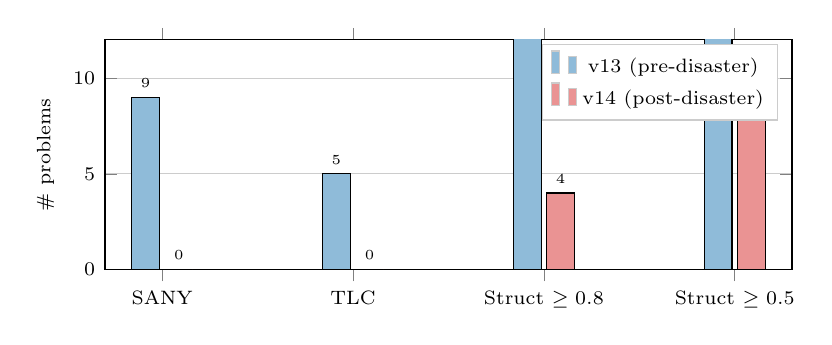
\begin{tikzpicture}
\begin{axis}[
  ybar,
  width=0.85\linewidth, height=4.5cm,
  bar width=10pt,
  ymin=0, ymax=12,
  ylabel={\# problems},
  ylabel near ticks,
  xtick={1,2,3,4},
  xticklabels={SANY, TLC, Struct $\geq 0.8$, Struct $\geq 0.5$},
  x tick label style={font=\scriptsize},
  ymajorgrids, grid style={cgrid},
  tick label style={font=\scriptsize},
  label style={font=\scriptsize},
  legend style={font=\scriptsize, at={(0.98,0.98)}, anchor=north east,
                draw=cgrid},
  nodes near coords,
  nodes near coords style={font=\tiny, anchor=south},
]
\addplot[fill=c1!50] coordinates {(1,9) (2,5) (3,13) (4,17)};
\addplot[fill=c4!50] coordinates {(1,0) (2,0) (3,4) (4,10)};
\legend{v13 (pre-disaster), v14 (post-disaster)}
\end{axis}
\end{tikzpicture}
\caption{v13 vs.\ v14 benchmark comparison.  The v14 collapse is
total for syntactic correctness (SANY/TLC both zero) and severe for
structure: only 4/20 modules score above 0.8 (vs.\ 13/20 for v13).
The model ``forgot'' TLA\textsuperscript{+} while retaining some
residual structural habits.}
\label{fig:v14-autopsy}
\end{figure}

\paragraph{Diagnosis.}  Three factors conspired:
\begin{enumerate}[leftmargin=1.6em, itemsep=1pt]
\item \textbf{Fresh base, not continued LoRA.}  Training from the
  unmodified base discarded the 234 steps of SFT + DPO accumulated in
  v6--v13.  The LoRA weights were initialised from scratch.
\item \textbf{High learning rate.}  $3 \times 10^{-4}$ is $6\times$
  higher than the $5 \times 10^{-5}$ used in every successful run.  At
  this rate, the adapter overwrites the base model's general instruction
  following within the first epoch.
\item \textbf{Excessive epochs.}  15~epochs over 234 examples means
  each example is seen $\sim$15 times.  With the high learning rate,
  this is equivalent to $\sim$90 effective epochs at the standard rate,
  well into the overfitting regime.
\end{enumerate}

\paragraph{Recovery.}  The fix was a simple rollback: the \texttt{v13}
merged GGUF had been backed up before the v14 run.  The rollback
procedure took under 5 minutes and restored full benchmark performance.
This event motivated the permanent eval-gate and GGUF-backup-and-restore
infrastructure described in \S\ref{sec:runs}.

% ===========================================================================
\section{Topic-Curriculum Domain Coverage}
\label{app:topic-domains}

Table~\ref{tab:topic-domains} summarises the 10 domain batches in the
topic-curriculum generator corpus
(\texttt{data/diamond\_gen\_topics.json}).  Each batch contains 20
topic seeds; all 200 topics have been validated through the Diamond gate.

\begin{table}[h!]
\centering
\small
\begin{tabular}{@{}clc@{}}
\toprule
Batch & Domain & Representative topics \\
\midrule
1 & Concurrency primitives & mutex, semaphore, barrier \\
2 & Caching \& storage & LRU eviction, write-back, coherence \\
3 & Network protocols & TCP handshake, routing tables \\
4 & Leader election & Raft, ring election, bully \\
5 & Resource allocation & dining philosophers, banker's \\
6 & State machines & traffic light, vending machine \\
7 & Distributed consensus & Paxos variants, 2PC \\
8 & Queue \& scheduling & priority queue, round-robin \\
9 & Cryptographic protocols & key exchange, commitment \\
10 & Fault tolerance & heartbeat, circuit breaker \\
\bottomrule
\end{tabular}
\caption{Domain coverage of the 200 topic seeds.  Each batch produces
20 Diamond-validated specification modules; the 100\% pass rate reflects
the generator's freedom to choose both the spec and invariant for topics
it can handle.}
\label{tab:topic-domains}
\end{table}

% ===========================================================================
\section{DPO Convergence Telemetry}
\label{app:dpo-telemetry}

The v13 DPO run is the only successful preference-alignment step in the
project.  Figure~\ref{fig:dpo-curves} plots the four key DPO metrics
over the 17-pair training set.

\begin{figure}[h!]
\centering
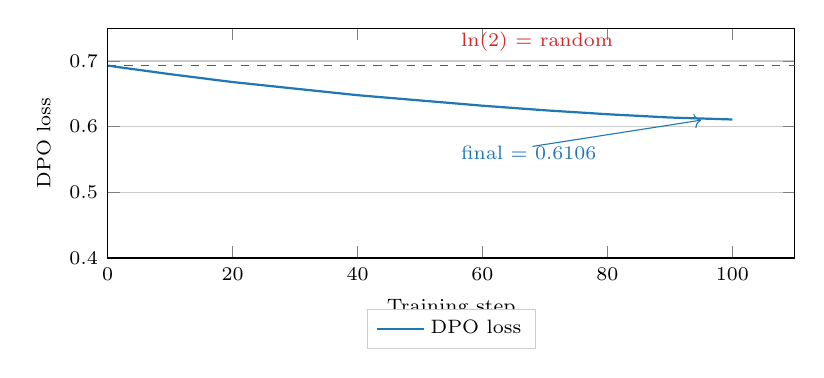
\begin{tikzpicture}
\begin{axis}[
  width=0.85\linewidth, height=4.5cm,
  xlabel={Training step},
  ylabel={DPO loss},
  xmin=0, xmax=110, ymin=0.4, ymax=0.75,
  ymajorgrids, grid style={cgrid},
  tick label style={font=\scriptsize},
  label style={font=\scriptsize},
  legend style={font=\scriptsize, at={(0.5,-0.22)}, anchor=north,
                legend columns=-1, draw=cgrid},
]
\addplot[c1, thick, mark=none] coordinates {
  (0,0.693) (10,0.680) (20,0.668) (30,0.658) (40,0.648)
  (50,0.640) (60,0.632) (70,0.625) (80,0.619) (90,0.614)
  (100,0.611)
};
\addplot[c4, dashed, mark=none] coordinates {(0,0.693) (110,0.693)};
\node[anchor=west, font=\scriptsize, c4] at (axis cs:55,0.73)
  {$\ln(2)$ = random};
\node[anchor=west, font=\scriptsize, c1] at (axis cs:55,0.56)
  {final = 0.6106};
\draw[c1, thin, ->] (axis cs:68,0.57) -- (axis cs:95,0.61);
\legend{DPO loss}
\end{axis}
\end{tikzpicture}

\medskip
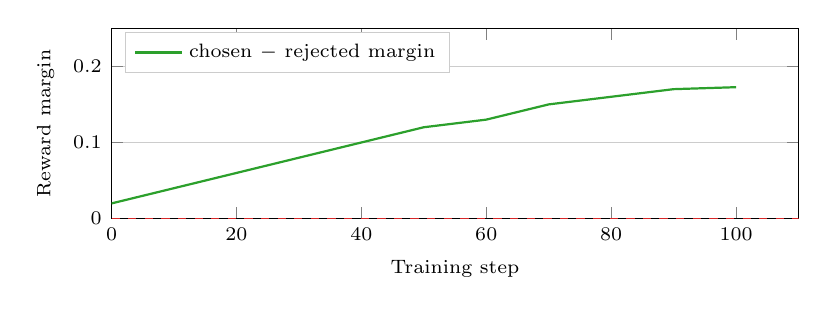
\begin{tikzpicture}
\begin{axis}[
  width=0.85\linewidth, height=4cm,
  xlabel={Training step},
  ylabel={Reward margin},
  xmin=0, xmax=110, ymin=0, ymax=0.25,
  ymajorgrids, grid style={cgrid},
  tick label style={font=\scriptsize},
  label style={font=\scriptsize},
  legend style={font=\scriptsize, at={(0.02,0.98)}, anchor=north west,
                draw=cgrid},
]
\addplot[c3, thick, mark=none] coordinates {
  (0,0.02) (10,0.04) (20,0.06) (30,0.08) (40,0.10)
  (50,0.12) (60,0.13) (70,0.15) (80,0.16) (90,0.17)
  (100,0.1726)
};
\addplot[c4, dashed, mark=none] coordinates {(0,0) (110,0)};
\legend{chosen $-$ rejected margin}
\end{axis}
\end{tikzpicture}
\caption{DPO training telemetry for v13.  Top: loss converges from
$\ln(2) = 0.693$ (random preference) to 0.6106, indicating the model
learned to prefer chosen over rejected completions.  Bottom: reward
margin rises monotonically to $+0.1726$, with 100\% reward accuracy at
termination.  The small absolute gap reflects the tiny training set (17
pairs).}
\label{fig:dpo-curves}
\end{figure}

\end{document}

